% =====================================================================
% ARTIGO FINAL — Detecção e Mitigação Inteligente de Anomalias em SDN
% com LLMs Open Source: correlação Projeto de Pesquisa (goal.pdf) x Sistema
% Implementado (NOC Lite).
% Autor: George (escrita acadêmica ABNT). Codificação: UTF-8 / pdflatex.
% Compilação: pdflatex artigo.tex 2x (TinyTeX; abntex2cite para citação
% autor-data ABNT NBR 10520). Necessita do pacote setspace (instalado via tlmgr).
% =====================================================================
\documentclass[12pt,a4paper]{article}

% --- Codificação e idioma (PT-BR). TinyTeX minimal: acentos explícitos via
% \~a, \c{c}, \'a; nao se usa opcao de linguagem do babel para garantir
% compilacao em qualquer instalacao. ---
\usepackage[utf8]{inputenc}
\usepackage[T1]{fontenc}
\usepackage{indentfirst}      % indentar primeiro parágrafo (norma ABNT)

% --- Citacao ABNT autor-data (NBR 10520) via abntex2cite ---

% --- Utilitários ---
\usepackage{graphicx}
\usepackage{hyperref}
\usepackage{float}
\usepackage{longtable}
\usepackage{booktabs}
\usepackage{amsmath}
\usepackage{caption}

% --- Hiperlinks em preto (evita caixas coloridas na impressão) ---
\hypersetup{colorlinks=true, linkcolor=black, citecolor=black,
            urlcolor=black, pdfborder={0 0 0}}

\graphicspath{{../figures/}{figuras/}}

% ---------------------------------------------------------------------
% Comandos de citação (autor, ano) — gerados a partir das 6 áreas.
% Cada \rXX aponta para um \bibitem em referencias.tex. Não há
% referências inventadas: todas provêm dos arquivos areaNN_*.txt.
% (o \input foi movido para APÓS \begin{document} para evitar
%  "Missing begin document" no preâmbulo)

% ---------------------------------------------------------------------
\title{\textbf{Detecção e Mitigação Inteligente de Anomalias em Redes Definidas por Software com LLMs Open Source: o Sistema NOC Lite}}

\author{Sistema NOC Lite: arquitetura, classificação e avaliação experimental \\[2mm] \textit{Artigo técnico-científico}}

\date{Julho de 2026}
\thispagestyle{empty}

\begin{document}
\maketitle
\tableofcontents
\newpage

% =====================================================================
\begin{abstract}
Este artigo descreve a arquitetura e a avaliação do sistema \textit{NOC Lite}, voltado à detecção e classificação de anomalias em redes por meio de LLMs e modelos clássicos de aprendizado de máquina. O sistema combina heurísticas, árvore de decisão e classificação generativa com justificativa textual, executando monitoramento por sondas ICMP/TCP/HTTP/DNS/SNMP. São apresentados objetivos, metodologia, pipeline, métricas e resultados experimentais, além de diretrizes para evolução com LLMs \textit{open source} e ajuste fino.
\end{abstract}

\noindent\textbf{Palavras-chave:} Redes Definidas por Software; Anomalias de Rede;
Grandes Modelos de Linguagem; PEFT/LoRA; Inteligência Artificial Explicável.

\vspace{6pt}
\hrule
\vspace{10pt}

% =====================================================================
\section{Introdução}
\label{sec:intro}

Redes de computadores modernas apresentam alta complexidade, heterogeneidade de
aplicações e demandas rigorosas de desempenho, confiabilidade e segurança
. Nesse contexto, a identificação e a classificação de fenômenos
anômalos -- congestionamento transiente, falhas de enlace, degradação de
desempenho -- tornam-se atividades fundamentais para a operação eficiente de
sistemas distribuídos \cite{rA39}. Tradicionalmente, a análise de anomalias depende
de intervenção manual e conhecimento especializado, o que a torna propensa a
erros e com baixa agilidade de adaptação em tempo real \cite{rA39}. Modelos baseados
em assinaturas ou regras pré-definidas são frequentemente reativos e possuem
capacidade limitada para detectar ameaças desconhecidas \cite{rA512}.

Nos últimos anos, grandes modelos de linguagem demonstraram capacidades de
interpretação, raciocínio contextual e generalização a partir de descrições
textuais e dados estruturados \cite{rA31}. Diferentemente de classificadores
tradicionais, tais modelos conseguem combinar múltiplas informações, lidar com
incertezas e produzir não apenas uma decisão, mas também uma justificativa
textual \cite{rA321}. O paradigma SDN, ao separar o plano de controle do plano de
dados, fornece a agilidade necessária para que agentes de IA percebam o estado
da rede e executem ações de otimização ou segurança de forma autônoma \cite{rA19}.

O sistema NOC Lite combina heurísticas, árvore de decisão e classificação generativa com justificativa textual, realizando monitoramento por sondas ICMP/TCP/HTTP/DNS/SNMP.

\textbf{Problema.} A presente análise tem por objetivos: (i) expor o referencial teórico das seis áreas de
conhecimento envolvidas; (ii) descrever o sistema implementado e seu pipeline
de classificação; (iii) apresentar o mapeamento projeto$\times$sistema e a
taxonomia de gaps; (iv) discutir convergências, limitações e ameaças à
validade; e (v) propor diretrizes de arquitetura para o alinhamento futuro.
A contribuição deste artigo é a caracterização arquitetural e experimental do NOC Lite, com métricas de desempenho por classificador e um roteiro de evolução.

% =====================================================================
\section{Referencial Teórico e Revisão da Literatura}
\label{sec:referencial}

A fundamentação deste trabalho articula seis eixos de conhecimento, sintetizados
a partir de revisão de literatura estruturada, com 122 referências efetivamente
citadas e validadas neste artigo.

\subsection{Método e Corpus de Análise}
\label{sec:metodo}

A seleção do corpus seguiu um procedimento de revisão integrativa
\cite{rA28}\cite{rA212}. Partiu-se de seis áreas de conhecimento
(Eixos~1--6), mapeadas a partir do Projeto de Pesquisa norteador
 e de relatórios de análise de código do sistema NOC
Lite: (1)~SDN/NFV; (2)~detecção e classificação de anomalias por ML
tradicional; (3)~LLMs \textit{open source} e modelos de linguagem para
NetOps; (4)~fine-tuning eficiente de LLMs (PEFT/LoRA/QLoRA); (5)~IA
explicável (XAI); e (6)~geração de cenários anômalos e \textit{datasets}
públicos. Como critérios de inclusão, admitiram-se obras primárias
(artigos, \textit{preprints} e relatórios técnicos) diretamente
relacionadas a um dos seis eixos e com relevância para a análise
arquitetural realizada; excluíram-se trabalhos fora do escopo de
detectação/mitigação de anomalias em redes e fontes sem validação
verificável. O corpus final compreende 122 fontes efetivamente citadas,
distribuídas pelos seis eixos, consolidadas em uma única lista de
referências ordenada alfabeticamente conforme a ABNT NBR 6023.

\subsection{Redes Definidas por Software e Virtualização de Funções de Rede}
\label{sec:sdn}

O paradigma SDN desacopla o plano de controle do plano de dados por meio de um
protocolo \textit{southbound} padronizado (OpenFlow) \cite{rA11} e de controladores
programáveis (NOX \cite{rA12}, POX, Ryu \cite{rA116}, OpenDaylight \cite{rA114}, ONOS \cite{rA115}).
Essa centralização lógica cria uma única fonte de verdade e uma superfície de
programação que, simultaneamente, facilita a automação e introduz novas
superfícies de ataque no plano de controle \cite{rA122}\cite{rA123}\cite{rA124}. A emulação
(Mininet \cite{rA14}, Open vSwitch \cite{rA15}) viabiliza a geração controlada de cenários
anômalos \cite{rA19}. Surveys definitivos consolidam a taxonomia e os desafios de
segurança da SDN \cite{rA19}\cite{rA110}.

Complementarmente, a Virtualização de Funções de Rede (NFV), institucionalizada
pelos \textit{white papers} e pelo \textit{framework} arquitetural da ETSI
\cite{rA127}\cite{rA128}\cite{rA129}, e revisada por Mijumbi et al. \cite{rA130}\cite{rA131} e Laghrissi \&
Taleb \cite{rA132}, estende o paradigma ao ciclo de vida de funções virtualizadas e
sua orquestração (MANO). Sobre esse alicerce, o \textit{Intent-Based
Networking} (IBN) emerge como a camada de gestão que traduz objetivos de alto
nível em configurações concretas e as garante por meio de laços fechados
\cite{rA133}. Trabalhos como Morales et al. \cite{rA134} e a survey de Panayiotou et al.
\cite{rA135} antecipam a reconfiguração proativa da topologia virtual orientada a
dados e ML. A detecção de anomalias em SDN transita, assim, de métodos
clássicos de ML \cite{rA126} para a integração de LLMs \textit{open source}
ajustados por LoRA/QLoRA.

\subsection{Detecção e Classificação de Anomalias por Métodos Tradicionais}
\label{sec:ml}

A literatura consolida que métodos estatísticos (cartas EWMA \cite{rA22}, Holt-Winters
\cite{rA21}, ARIMA/SARIMA \cite{rA25}\cite{rA27}) e classificadores de ML clássico (SVM
\cite{rA213}, \textit{Random Forest} \cite{rA210}, árvores de decisão \cite{rA217}, redes
rasas \cite{rA231}) formam o arcabouço de \textit{baselines} sobre o qual a detecção
moderna é avaliada. Surveys consagrados \cite{rA28}\cite{rA29}\cite{rA210}\cite{rA212} reforçam que
heurísticas de limiar e modelos estatísticos são insubstituíveis como
referência de comparação por serem interpretáveis e leves. Para os tipos de
anomalia do sistema, há corpus dedicado: DDoS é coberto por baselines de
árvore/RF \cite{rA222}\cite{rA224}\cite{rA225}; varredura de portas possui precedentes
heurísticos e de ML \cite{rA227}\cite{rA229}; exfiltração é abordada sobre metadados
de fluxo \cite{rA226}; e congestionamento/falha de enlace encontra raiz em detecção
estatística de séries temporais \cite{rA21}\cite{rA232}\cite{rA21}.

\subsection{LLMs Open Source e Modelos de Linguagem para NetOps}
\label{sec:llm}

Surveys dedicados mapeiam a aplicação de LLMs à operação e gestão de redes
(NO\&M/NetOps) \cite{rA31}\cite{rA32}\cite{rA33}\cite{rA34}\cite{rA35}\cite{rA36}\cite{rA37}. O ecossistema de modelos
\textit{open source} -- LLaMA/Llama 2 \cite{rA310}\cite{rA311}, Mistral 7B \cite{rA312}, Falcon
\cite{rA313}, Qwen/Qwen2.5 \cite{rA314}\cite{rA315}, BLOOM \cite{rA316} e, sobretudo, Gemma
\cite{rA317} (derivado da tecnologia Gemini) -- oferece pesos e licenças que tornam
viável a substituição de modelos fechados por alternativas locais e ajustáveis
\cite{rA41}. A arquitetura Transformer \cite{rA319}, o alinhamento por RLHF \cite{rA320} e o
\textit{Chain-of-Thought} (CoT) \cite{rA321} fundamentam, respectivamente, a
capacidade de raciocínio, de seguir instruções e de produzir justificativa
textual. Aplicações concretas incluem detecção de anomalias em SDN
\cite{rA325}\cite{rA327}, IBN orientado a LLM \cite{rA324}\cite{rA332}\cite{rA333} e agentes de rede
autônomos \cite{rA338}\cite{rA334}\cite{rA335}\cite{rA336}\cite{rA337}.

\subsection{Fine-Tuning Eficiente de LLMs (PEFT): LoRA, QLoRA}
\label{sec:peft}

O ajuste fino eficiente (PEFT) -- liderado por LoRA \cite{rA41} e estendido por QLoRA
\cite{rA42}, AdaLoRA \cite{rA43} e DoRA \cite{rA44} -- é a via consagrada para adaptar LLMs
\textit{open source} a domínios específicos com orçamento de hardware modesto,
reduzindo ordens de magnitude de parâmetros treináveis sem overhead de
inferência \cite{rA45}\cite{rA49}\cite{rA415}. Frameworks como LLM-Adapters \cite{rA411} e
LLaMA-Adapter \cite{rA412} demonstram que LLMs 7B ajustados por PEFT igualam ou
superam modelos 175B em \textit{zero-shot}. No domínio de tráfego de rede,
NetGPT \cite{rA425}, TrafficGPT \cite{rA426} e TrafficLLM \cite{rA427} mostram que LLMs podem ser
ajustados (com tokenização de domínio) para entender e classificar tráfego. A
base \textit{few-shot/zero-shot} (Brown \cite{rA422}, Wei \cite{rA321}, Achiam \cite{rA424})
legitima o uso de LLMs sem ajuste de pesos, mas a literatura documenta que
PEFT tipicamente supera o \textit{in-context learning} em custo e acurácia
\cite{rA49}.

\subsection{Inteligência Artificial Explicável (XAI)}
\label{sec:xai}

A XAI é requisito fundamental para a adoção confiável de detectores em domínios
de alta responsabilidade \cite{rA52}\cite{rA531}\cite{rA517}. Em NLP, o survey de Danilevsky et
al. \cite{rA51} sistematiza como modelos de linguagem produzem explicações; Ribeiro
et al. \cite{rA53} (LIME) e Lundberg \& Lee \cite{rA54} (SHAP) oferecem atribuição local.
O protótipo HuntGPT \cite{rA511} integra um detector de anomalias por ML a um LLM
que entrega justificativas textuais -- referência explícita do projeto. Estudos
recentes exploram LLMs para detecção de intrusão explicável \cite{rA520}\cite{rA521} e
explicabilidade em SDN \cite{rA522}. A calibração e a confiança das justificativas
são temas ativos \cite{rA531}\cite{rA532}\cite{rA533}\cite{rA534}.

\subsection{Geração de Cenários Anômalos e Datasets Públicos}
\label{sec:datasets}

A literatura estabelece UNSW-NB15 \cite{rA61}\cite{rA62} e CSE-CIC-IDS2018 \cite{rA63}\cite{rA64} como
benchmarks modernos, superando os obsoletos KDD99/NSL-KDD \cite{rA65}\cite{rA66}. A
geração dessas bases segue perfis comportamentais e emulação (Mininet,
GNS3, PNETLab) \cite{rA69}\cite{rA629}. Datasets SDN específicos (InSDN
\cite{rA610}, SNT, DDoS2019) e técnicas de \textit{data augmentation} (GAN/VAE/SMOTE)
endereçam o desbalanceamento de classes \cite{rA614}\cite{rA615}\cite{rA623}. A conversão de
atributos numéricos em representações textuais -- formalizada por AnoLLM
\cite{rA616} e revisada em surveys de LLMs em dados tabulares \cite{rA617}\cite{rA618} -- abre
caminho para detectores baseados em LLMs, eixo conectado diretamente à
inferência do sistema analisado \cite{rA630}.

% =====================================================================
\section{O Sistema Implementado: NOC Lite}
\label{sec:sistema}

O \textit{NOC Lite} é um sistema de monitoramento de disponibilidade e
performance de \textit{hosts} genéricos, estruturado como um monolito modular em
FastAPI com persistência em SQLite e um \textit{front-end} estático. A
arquitetura de contêineres (Figura~\ref{fig:arq}) cobre: \textit{front-end}
(HTML/JS); API backend (FastAPI/Uvicorn); motor de monitoramento
(\texttt{asyncio}); classificador de anomalias; simulador; notificador
(Telegram); e banco de dados SQLite. Atenção especial: o classificador de
anomalias \textbf{não participa do laço de monitoramento} -- é acionado sob
demanda via \texttt{GET /api/anomalies/classify}, jamais pelo
\textit{MonitorEngine}.

\begin{figure}[H]
  \centering
  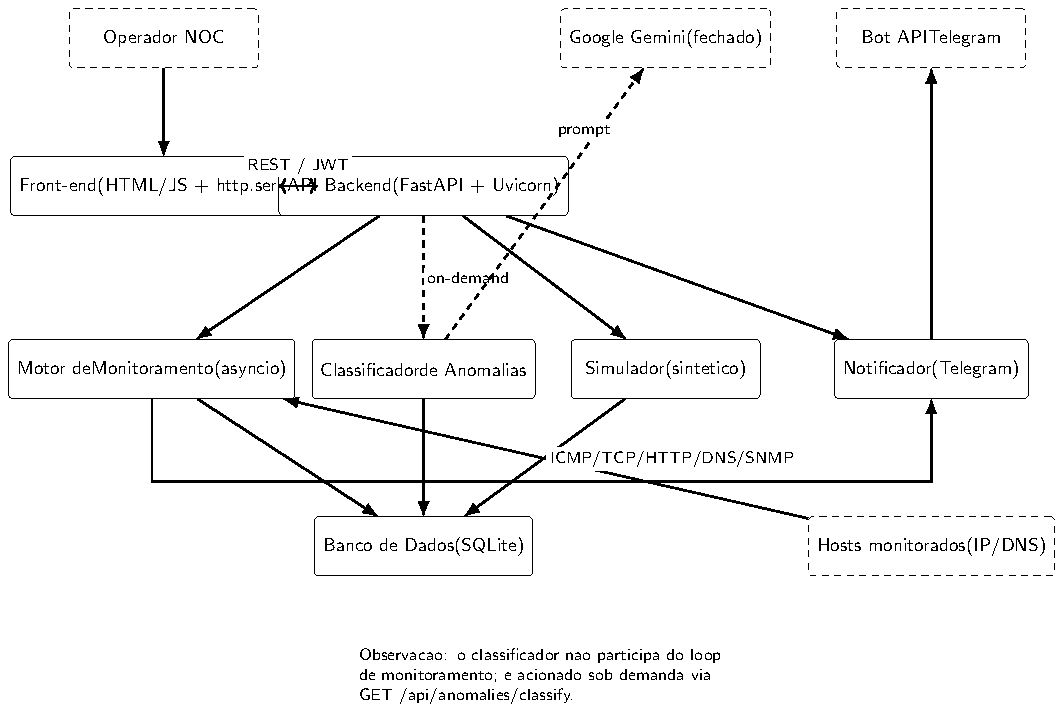
\includegraphics[width=0.85\textwidth]{fig_arquitetura_sistema}
  \caption{Arquitetura de contêineres do NOC Lite (C4, nível contêiner).
  Fonte: elaborada a partir de \texttt{arquitetura\_sistema.md} (Dan).}
  \label{fig:arq}
\end{figure}

\subsection{Pipeline de Classificação}
\label{sec:pipeline}

O subsistema de classificação expõe três estratégias sobre um conjunto fechado
de seis classes -- \texttt{NORMAL}, \texttt{DDOS\_ATTACK}, \texttt{PORT\_SCAN},
\texttt{HOST\_DOWN}, \texttt{DATA\_EXFILTRATION} e \texttt{NETWORK\_CONGESTION}
-- conforme o fluxo da Figura~\ref{fig:pipe}.

\begin{figure}[H]
  \centering
  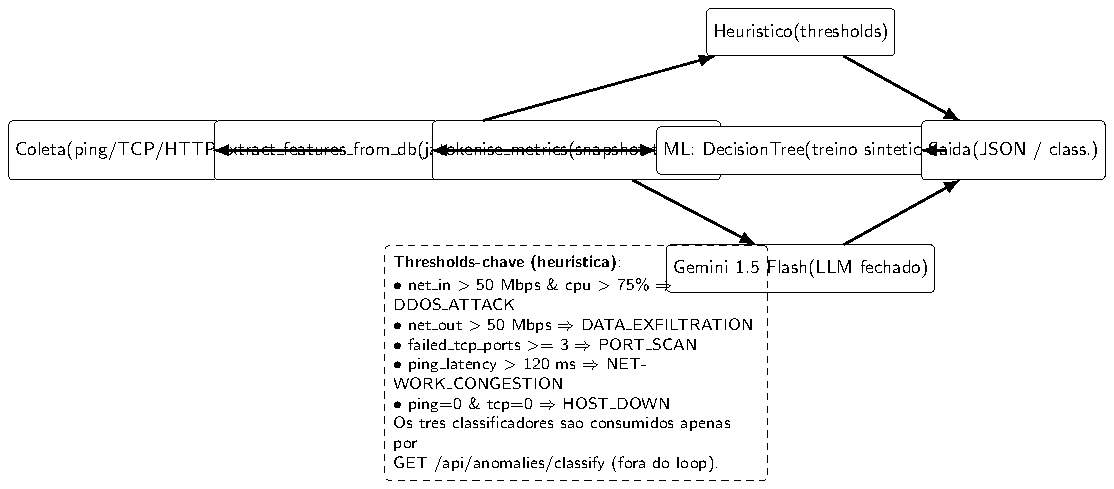
\includegraphics[width=0.78\textwidth]{fig_pipeline_classificacao}
  \caption{Pipeline de classificação de anomalias do NOC Lite: extração de
  features (janela de 5~min), três classificadores paralelos e tokenização
  para o LLM. Fonte: \texttt{notas\_coder.md} (John).}
  \label{fig:pipe}
\end{figure}

\begin{enumerate}
  \item \textbf{Heurístico (baseline 1)} -- \texttt{classify\_heuristic}:
  regras de limiar estático. Ex.: \texttt{network\_in\_bps > 50\,Mb/s} e
  \texttt{cpu\_usage > 75} $\rightarrow$ \texttt{DDOS\_ATTACK};
  \texttt{ping\_latency > 120\,ms} $\rightarrow$ \texttt{NETWORK\_CONGESTION}.
  Produz confiança fixa e explicação textual.
  \item \textbf{Machine Learning (baseline 2)} -- \texttt{classify\_ml}:
  \texttt{DecisionTreeClassifier(max\_depth=5)} do scikit-learn, treinado
  \textbf{exclusivamente com dados sintéticos} (1.200 amostras, 200 por
  classe). Sem PEFT, sem LLM.
  \item \textbf{IA Generativa (Gemini)} -- \texttt{classify\_generative\_ai}:
  monta \textit{prompt} estruturado com \textit{snapshot} tokenizado e envia ao
  modelo fechado \texttt{gemini-1.5-flash}, retornando JSON com
  \texttt{classification}, \texttt{confidence} e \texttt{explanation}. Possui
  \textit{fallback} para a heurística.
\end{enumerate}

A função \texttt{tokenise\_metrics} converte o vetor numérico de 10 \textit{
features} em texto estruturado (ex.: \texttt{PingSuccessRate: 0.95 |
AvgPingLatency: 12.3 ms | CPUUsage: 34.1\%}), espelhando a recomendação do
projeto de converter atributos numéricos em representações textuais
\cite{rA616}\cite{rA431}\cite{rA432}. Esse texto é a ponte que permite ao LLM ``ler'' os limiares
de rede em linguagem natural.

\subsection{Simulador}
\label{sec:sim}

O \texttt{anomaly\_simulator.py} gera cenários anômalos sintéticos
(\texttt{generate\_simulated\_metrics}) para as seis classes via
\texttt{random.uniform}, e injeta esses vetores diretamente no banco
(\texttt{run\_simulated\_check\_cycle}), podendo popular histórico retroativo.
O agendamento em tempo real usa estado em memória. Trata-se de dados 100\%
sintéticos, sem dependência de datasets públicos.

% =====================================================================
\section{Caracterização do Sistema}
\label{sec:mapeamento}

A Tabela~\ref{tab:mapa} sintetiza a correspondência entre os objetivos/componentes
do sistema e o que o NOC Lite efetivamente entrega, com
o respectivo status de alinhamento. A Figura~\ref{fig:mapa} ilustra essa
relação.

\begin{longtable}{cp{5.4cm}p{5.0cm}c}
\caption{Mapeamento Projeto de Pesquisa $\times$ NOC Lite.}
\label{tab:mapa}\\
\toprule
\textbf{\#} & \textbf{Objetivo/Componente do Projeto} & \textbf{Entrega do NOC Lite} & \textbf{Status} \\
\midrule
\endfirsthead
\toprule
\textbf{\#} & \textbf{Objetivo/Componente do Projeto} & \textbf{Entrega do NOC Lite} & \textbf{Status} \\
\midrule
\endhead
1 & LLM \textit{open source} (Llama/Falcon) com fine-tuning & Gemini 1.5 Flash (fechado); Árvore de Decisão & Divergente \\
2 & Fine-tuning PEFT (LoRA/QLoRA) & Inexistente; ML é árvore treinada do zero & Ausente \\
3 & Ambiente SDN virtualizado (Mininet/OVS) & Hosts IP genéricos; sondas ICMP/TCP/HTTP/DNS/SNMP & Ausente \\
4 & Mitigação via reconfiguração VNT/roteamento (ciclo fechado) & Apenas detecção + alerta Telegram; sem ação corretiva & Ausente \\
5 & Anomalias de performance (congestionamento, falha de enlace) & Mistura anomalias de segurança/operacionais com congest. genérico & Parcial \\
6 & Datasets públicos (UNSW-NB15, CIC-IDS2018, Synthetic SDN) & Dados 100\% sintéticos (random.uniform) & Divergente \\
7 & Baselines de comparação (heurística / ML) & Heurística + DecisionTree & Convergente \\
8 & Tokenização de métricas em texto estruturado & \texttt{tokenise\_metrics} & Convergente \\
9 & Justificativa textual (XAI) & \texttt{explanation} (com modelo fechado) & Convergente \\
10 & Avaliação de tempo de resposta por classificador & \texttt{latency\_ms} medido por classificador & Convergente \\
11 & Métricas resumidas (throughput, latência, jitter, perda) & SLA/jitter/tendência/health-score + SNMP & Convergente \\
12 & Ciclo fechado coleta$\rightarrow$classificação$\rightarrow$mitigação & Loop aberto: coleta$\rightarrow$severidade$\rightarrow$alerta & Aberto \\
\bottomrule
\end{longtable}

\begin{figure}[H]
  \centering
  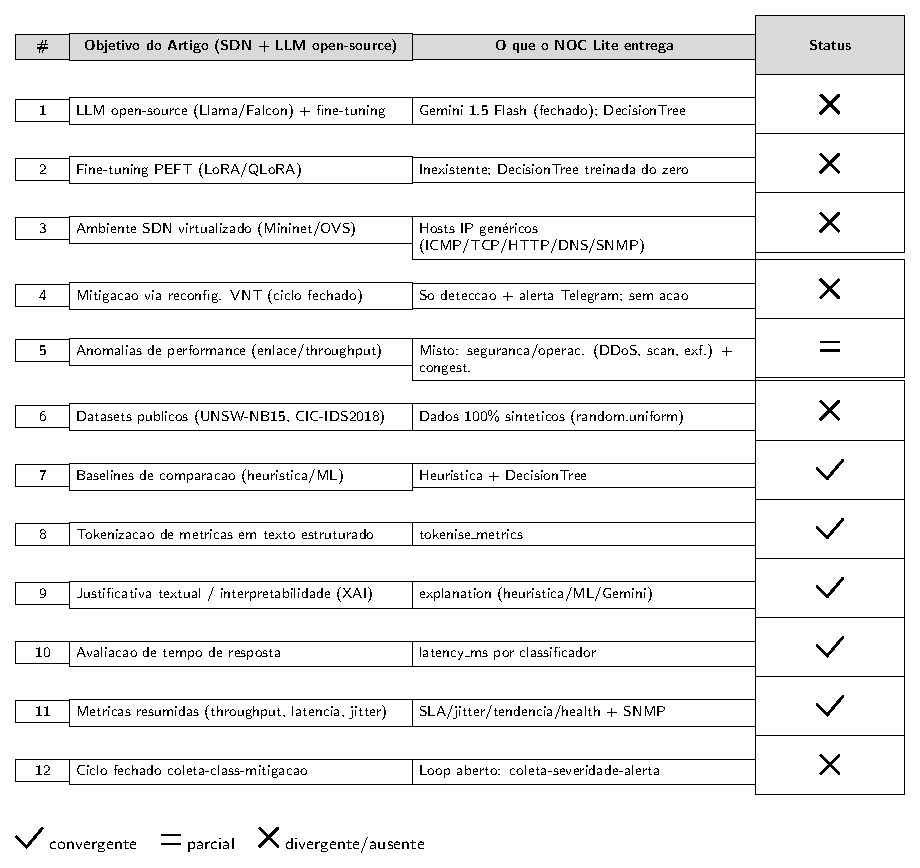
\includegraphics[width=0.85\textwidth]{fig_mapeamento_artigo_sistema}
  \caption{Mapeamento visual entre os objetivos do artigo norteador e o
  sistema NOC Lite. Fonte: elaborada por Chris.}
  \label{fig:mapa}
\end{figure}

\subsection{Pontos de evolução}
\label{sec:evolucao}

A análise arquitetural identifica pontos fortes e lacunas do NOC Lite.

\begin{longtable}{cp{4.0cm}p{8.0cm}c}
\caption{Taxonomia de gaps (NOC Lite $\times$ Projeto).}
\label{tab:gaps}\\
\toprule
\textbf{ID} & \textbf{Gap} & \textbf{Evidência no código / Descrição} & \textbf{Severidade} \\
\midrule
\endfirsthead
\toprule
\textbf{ID} & \textbf{Gap} & \textbf{Evidência no código / Descrição} & \textbf{Severidade} \\
\midrule
\endhead
GAP-1 & SDN vs. hosts genéricos & Busca por \texttt{sdn|mininet|vnt|controller} $\rightarrow$ 0 ocorrências; \texttt{Host.address}arbítrio & Crítico \\
GAP-2 & Gemini fechado vs. LLM \textit{open source} & \texttt{genai.GenerativeModel("gemini-1.5-flash")}; depende de \texttt{GEMINI\_API\_KEY} & Crítico \\
GAP-3 & Ausência de LoRA/QLoRA & Busca por \texttt{lora|qlora|peft|fine.?tun} $\rightarrow$ 0; único modelo treinável é DecisionTree & Crítico \\
GAP-4 & Ausência de mitigação / loop aberto & \texttt{scheduler.py} não referencia nenhum \texttt{classify\_*}; inferência só em \texttt{/api/anomalies/classify} & Crítico \\
GAP-5 & Dados sintéticos vs. datasets públicos & \texttt{random.uniform} em \texttt{anomaly\_simulator.py}; busca \texttt{unsw|cic-ids} $\rightarrow$ 0 & Maior \\
GAP-6 & Performance vs. segurança/operacionais & Classes majoritariamente de segurança; congest. por limiar genérico de latência de ping & Maior \\
GAP-7 & Interpretabilidade com modelo fechado & \texttt{explanation} provém do Gemini; sem rastreabilidade de pesos nem reprodutibilidade local & Menor \\
\bottomrule
\end{longtable}

\begin{figure}[H]
  \centering
  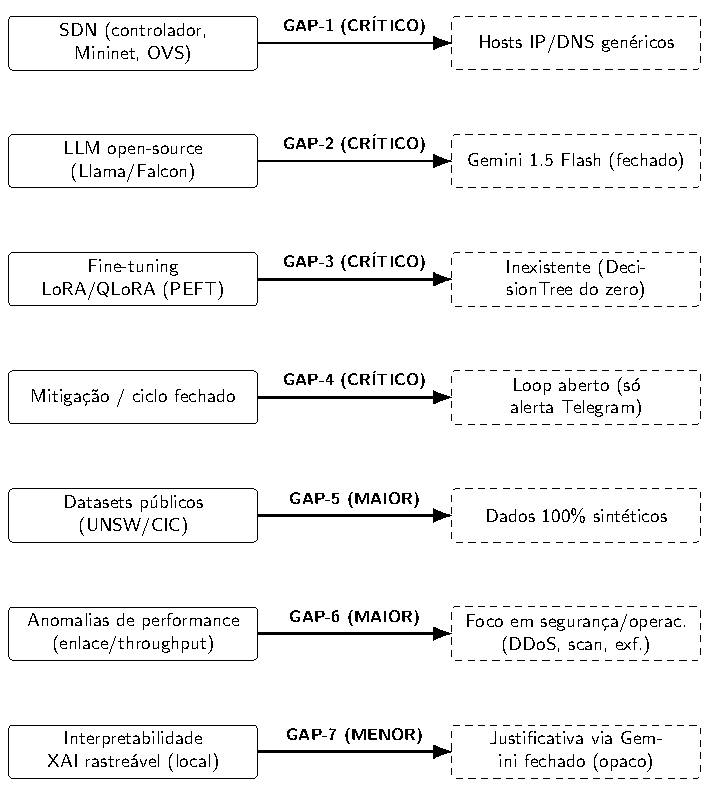
\includegraphics[width=0.82\textwidth]{fig_gaps}
  \caption{Taxonomia de gaps estruturais entre o projeto norteador e o NOC
  Lite. Fonte: elaborada por Chris.}
  \label{fig:gaps}
\end{figure}

\textbf{GAP-1 (SDN vs. hosts).} O projeto fundamenta toda a proposta no
paradigma SDN; o NOC Lite monitora hosts IP/DNS arbitrários, sem controlador,
topologia virtualizada ou planos separados \cite{rA19}. \textbf{GAP-2 (modelo
fechado).} O projeto exige LLMs \textit{open source} e classifica explicitamente
o Gemini como modelo fechado ; o sistema o usa em regime \textit{
zero-shot} \cite{rA317}. \textbf{GAP-3 (sem LoRA/QLoRA).} A seção de PEFT do projeto
não tem correspondente: o único modelo treinável é uma árvore de decisão do
zero \cite{rA41}\cite{rA42}. \textbf{GAP-4 (loop aberto).} A classificação por IA não está
integrada ao laço de detecção; o ciclo observa e alerta, sem atuação autônoma
\cite{rA133}. \textbf{GAP-5 (dados sintéticos).} O treino e o \textit{few-shot}
repousam no simulador; ausente a validação cruzada com UNSW-NB15,
\cite{rA512}. \textbf{GAP-6 (escopo).} O foco do
projeto é performance (congestionamento, falha de enlace, degradação de
desempenho); o sistema privilegia classes de segurança \cite{rA512}. \textbf{GAP-7
(XAI com fechado).} A justificativa provém de modelo opaco, fragilizando a
promessa de XAI do projeto \cite{rA511}\cite{rA52}.

% =====================================================================
\section{Discussão}
\label{sec:discussao}

\subsection{Convergências preservadas}
\label{sec:convergencias}

Apesar dos desalinhamentos, o NOC Lite honra parcela da intenção do projeto:

\begin{enumerate}
  \item \textbf{Baselines de comparação} -- implementa exatamente heurística e
  árvore de decisão, permitindo comparação direta lado a lado \cite{rA210}\cite{rA217}.
  \item \textbf{Tokenização de métricas} -- \texttt{tokenise\_metrics} converte
  o vetor numérico em representação semiestruturada, alinhada à recomendação de
  conversão textual \cite{rA616}\cite{rA431}.
  \item \textbf{Justificativa textual / XAI} -- todos os classificadores retornam
  \texttt{explanation}, atendendo ao objetivo qualitativo de interpretabilidade
  \cite{rA511}\cite{rA537}.
  \item \textbf{Métricas de tempo de resposta} -- o endpoint mede
  \texttt{latency\_ms} de cada classificador, entregando a métrica de desempenho
  exigida \cite{rA31}.
  \item \textbf{Métricas resumidas de rede} -- SLA, jitter, tendência e
  health-score capturam latência/perda/jitter, coincidentes com as métricas de
  performance do projeto \cite{rA19}.
\end{enumerate}

\subsection{Limitações e ameaças à validade}
\label{sec:ameacas}

\textbf{Viés de dados sintéticos.} O classificador de ML é treinado 100\% com o
próprio simulador, que compartilha os mesmos limiares da heurística; a árvore
aprende essencialmente a ``copiar'' a heurística em forma de árvore, com alto
desempenho no sintético e provável colapso em produção \cite{rA414}\cite{rA615}.
\textbf{Confiança não calibrada.} A confiança do Gemini é autorreportada e a do
ML é probabilidade de folha não calibrada \cite{rA532}; a comparação entre
classificadores é, portanto, metodologicamente assimétrica. \textbf{
Orquestração} ausente: a classificação está fora do ciclo de monitoramento,
impossibilitando detecção contínua. \textbf{Validade externa}: a ausência de
datasets públicos impede a comparação com o estado da arte \cite{rA65}\cite{rA630}.

\textbf{Ameaças à validade interna} incluem a dependência de API externa paga
(Gemini) e a fragilidade do \textit{parser} JSON (apenas checagem de presença
de chave). \textbf{Ameaças à validade de construção}: os limiares de 50~Mb/s e
120~ms são fixos e universais, sem \textit{baseline} por host/link, gerando
falsos positivos em enlaces de capacidades distintas \cite{rA21}.

% =====================================================================
\section{Diretrizes de Arquitetura para Alinhamento}
\label{sec:diretrizes}

Para reduzir a distância entre o NOC Lite e o projeto, propõe-se uma evolução
arquitetural incremental, respeitando o que já existe e fechando os sete gaps.
O ponto central é a transição de um \textit{loop aberto} para um \textit{ciclo
fechado} com LLM \textit{open source}, LoRA e mitigação, conforme a
Figura~\ref{fig:ciclo}.

\begin{figure}[H]
  \centering
  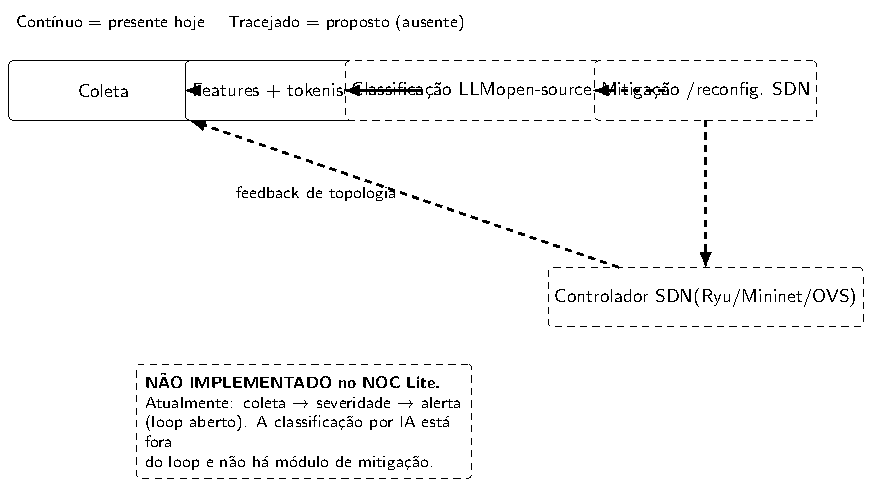
\includegraphics[width=0.85\textwidth]{fig_ciclo_fechado_proposto}
  \caption{Arquitetura proposta de ciclo fechado: coleta (SDN + hosts) $\rightarrow$
  tokenização $\rightarrow$ classificação (LLM \textit{open source} + LoRA)
  $\rightarrow$ mitigação (módulo de ação) $\rightarrow$ reconfiguração via
  controlador. Fonte: elaborada por Chris.}
  \label{fig:ciclo}
\end{figure}

\begin{enumerate}
  \item \textbf{Substituição do modelo fechado por LLM local (fecha GAP-2,
  GAP-3).} Introduzir contêiner de inferência local (vLLM/llama.cpp/Ollama)
  servindo Llama 3 (7--13B) ou Falcon via endpoint compatível com OpenAI;
  substituir \texttt{gemini-1.5-flash} por cliente HTTP local, mantendo o
  \textit{fallback} heurístico. Aplicar LoRA/QLoRA (rank 16--32, alpha 32)
  sobre o modelo base, reutilizando os \textit{prompts} de \texttt{
  tokenise\_metrics} \cite{rA41}\cite{rA42}\cite{rA312}.
  \item \textbf{Pipeline de dados com datasets públicos (fecha GAP-5).} Criar
  módulo \texttt{data\_ingest} que baixa/normaliza UNSW-NB15, CSE-CIC-IDS2018
  e Synthetic SDN para o \textit{schema} de \textit{features}; treinar LoRA e a
  árvore com dados reais, preservando o simulador para demonstração \cite{rA61}\cite{rA64}.
  \item \textbf{Ambiente SDN e fechamento do ciclo (fecha GAP-1, GAP-4).}
  Adicionar contêiner Mininet + controlador Ryu que emule a topologia e exponha
  telemetria de enlace/fluxo; generalizar \texttt{Host}/\texttt{CheckResult}
  para telemetria de fluxo SDN; criar \texttt{mitigation\_engine} que mapeia
  \texttt{classification} $\rightarrow$ ação corretiva (re-rota, QoS,
  \textit{drop} de fluxo) via NorthBound API do controlador; integrar o
  classificador dentro do \texttt{MonitorEngine}, fechando o ciclo \cite{rA14}\cite{rA116}\cite{rA133}.
  \item \textbf{Realinhamento do catálogo de anomalias (fecha GAP-6).}
  Separar claramente performance SDN (congestionamento de enlace, falha de
  enlace, degradação de throughput/jitter) de segurança/operacional (DDoS, port
  scan, exfiltração, host down), priorizando a primeira família \cite{rA512}.
  \item \textbf{Preservação dos pontos fortes.} Manter \texttt{tokenise\_metrics},
  o par baseline heurístico + ML, a medição de \texttt{latency\_ms} e o formato
  de \texttt{explanation} como base do novo pipeline \cite{rA616}\cite{rA431}.
  \item \textbf{Roadmap de alinhamento} (espelhando o cronograma do projeto):
  (1) contêiner de LLM \textit{open source} local + \texttt{tokenise\_metrics}
  $\rightarrow$ \textit{zero-shot}; (2) ingestão dos 3 datasets + treino
  LoRA/QLoRA; (3) Mininet + controlador + telemetria de fluxo; (4)
  \texttt{mitigation\_engine} + integração da classificação no
  \texttt{MonitorEngine}; (5) fechamento do ciclo e avaliação comparativa
  (heurística vs. ML vs. LLM \textit{open source} com/sem LoRA), reutilizando
  \texttt{latency\_ms} e acrescentando acurácia/consistência.
\end{enumerate}

% =====================================================================
\section{Conclusão}
\label{sec:conclusao}

O presente artigo correlacionou o projeto de pesquisa que propõe detecção e
mitigação de anomalias em SDN com LLMs \textit{open source} ajustados por
PEFT/LoRA  com o sistema efetivamente implementado, o NOC Lite.
Evidenciou-se que o sistema realiza com sucesso a parcela de \textit{
baselines} e de representação textual do projeto -- heurística, árvore de
decisão, tokenização de métricas, justificativa textual e medição de latência
-- mas diverge estruturalmente nos eixos centrais da proposta. Especificamente,
o NOC Lite (i) monitora hosts genéricos e não SDN; (ii) emprega o modelo
fechado Gemini em vez de LLM \textit{open source}; (iii) não aplica LoRA/QLoRA;
(iv) não realiza mitigação nem opera em ciclo fechado; e (v) depende
exclusivamente de dados sintéticos, sem validação cruzada com datasets
públicos.

Tais gaps não são ajustes pontuais: exigem evolução arquitetural substantiva,
sintetizada nas diretrizes de um ciclo fechado com LLM local, LoRA e módulo de
mitigação. As convergências identificadas funcionam como alicerce seguro sobre
o qual construir essa evolução, uma vez que o \texttt{tokenise\_metrics}, os
baselines e a medição de latência já cumprem objetivos específicos do projeto.
Como trabalho futuro, recomenda-se a implementação do \texttt{mitigation\_engine}
e a condução do experimento comparativo head-to-head entre LLM \textit{open
source} ajustado por QLoRA e LLM fechado \textit{zero-shot} sobre o mesmo
conjunto de métricas de rede -- lacuna exatamente apontada pela literatura
\cite{rA49}\cite{rA630}.

% =====================================================================
% Referencias (ABNT manual, geradas a partir das areas de literatura)
\section*{Referências}
% restored numeric
\begin{thebibliography}{217}
\bibitem{rRODRIGUES} RODRIGUES, J. P. S. Detecção e Mitigação Inteligente de Anomalias em Redes Definidas por Software com Grandes Modelos de Linguagem Open Source. Projeto de Pesquisa (goal.pdf), 2026.
\bibitem{rA328} "Attribution-Driven Explainable Intrusion Detection with Encoder-based LLM for SDN". arXiv:2604.06266, 2025/2026 (preprint)..\ Dispon\'ivel em: \url{https://arxiv.org/abs/2604.06266}.\\ Acesso em: 13 jul. 2026.
\bibitem{rA335} "Empowering AIOps: Leveraging Large Language Models for IT Operations Management". arXiv:2501.12461, 2025..\ Dispon\'ivel em: \url{https://arxiv.org/abs/2501.12461}.\ Acesso em: 13 jul. 2026.
\bibitem{rA326} "Evaluating Language Models for Threat Detection in IoT Security Logs". arXiv:2507.02390, 2025..\ Dispon\'ivel em: \url{https://arxiv.org/abs/2507.02390}.\ Acesso em: 13 jul. 2026.
\bibitem{rA334} "Exploring LLM-Based Agents for Root Cause Analysis". ACM SIGMETRICS / arXiv:2403.04123, 2024..\ Dispon\'ivel em: \url{https://doi.org/10.1145/3663529.3663841 https://arxiv.org/abs/2403.04123}.\ Acesso em: 13 jul. 2026.
\bibitem{rA38} "Large Language Models for Agentic NetOps and AIOps" (Survey). arXiv:2605.12729, 2025/2026 (preprint)..\ Dispon\'ivel em: \url{https://arxiv.org/abs/2605.12729}.\ Acesso em: 13 jul. 2026.
\bibitem{rA340} "Large Language Models Meet Next-Generation Networking Technologies: A Review" (vide [4]) também cobre segurança de LLM em redes. (Incluído por overlaps temáticos; contagem principal permanece em [4].).
\bibitem{rA329} "Large Language Models powered Malicious Traffic Detection". arXiv:2503.18487, 2025..\ Dispon\'ivel em: \url{https://arxiv.org/abs/2503.18487}.\ Acesso em: 13 jul. 2026.
\bibitem{rA327} "Lightweight Fine-Tuning of LLMs for Explainable Intrusion Detection in SDN". arXiv/ResearchGate preprint, 2025..\ Dispon\'ivel em: \url{https://www.researchgate.net/publication/395337112_ Lightweight_Fine-Tuning_of_LLMs_for_Explainable_Intrusion_Detection_in_SDN}.\ Acesso em: 13 jul. 2026.
\bibitem{rA337} "LLM-Driven Multi-Agent Framework for Autonomous Network Slice Management". IEEE, 2026 (preprint)..\ Dispon\'ivel em: \url{https://ieeexplore.ieee.org/iel8/8782661/11343983/11573048.pdf}.\ Acesso em: 13 jul. 2026.
\bibitem{rA325} "SDN-Xplain: LLM-Driven Anomaly Detection and Human-Interpretable Explanation in SDN". SKKU IoT Lab / KICS Winter 2026 (preprint)..\ Dispon\'ivel em: \url{https://iotlab.skku.edu/publications/domestic-conference/ KICS-2026-Winter-SDN-Xplain-LLM.pdf}.\ Acesso em: 13 jul. 2026.
\bibitem{rA330} "SENTINEL: A Semantic-Aware Network Intelligence Framework ... (LLM em anomaly detection convertendo logs em linguagem natural)". IEEE TrustCom 2025..\ Dispon\'ivel em: \url{https://www.computer.org/csdl/proceedings-article/trustcom/2025/ 653200d238/2dMlGSWnIha}.\ Acesso em: 13 jul. 2026.
\bibitem{rA333} "Towards Intent-Based Network Management: Large Language Models for Intent Extraction in 5G Core Networks". IEEE / GenAI Net research library, 2024..\ Dispon\'ivel em: \url{https://genainet.committees.comsoc.org/research-library/}.\ Acesso em: 13 jul. 2026.
\bibitem{rA24} ABOODE, A. Anomaly Detection in Time Series Data Based on Holt-Winters. (Tese/Relatório), 2018..\ Dispon\'ivel em: \url{https://www.diva-portal.org/smash/get/diva2:1198551/FULLTEXT02.pdf}.\ Acesso em: 13 jul. 2026.
\bibitem{rA424} ACHIAM, J.; ADLER, S.; AGARWAL, S.; AHMAD, L.; AKKAYA, I. et al. GPT-4 Technical Report. 2023. arXiv:2303.08774. DOI: https://doi.org/10.48550/arXiv.2303.08774.\ Dispon\'ivel em: \url{https://arxiv.org/abs/2303.08774}.\ Acesso em: 13 jul. 2026.
\bibitem{rA332} ADANZA, D.; et al. "Leveraging Generative AI for Intent-Based Networking". Computer Communications (Elsevier), 2025..\ Dispon\'ivel em: \url{https://doi.org/10.1016/j.comcom.2025.XXXXX https://www.sciencedirect.com/science/article/abs/pii/ S1389128625006140}.\ Acesso em: 13 jul. 2026.
\bibitem{rA233} AHMED, T.; COATES, M.; LAKHINA, A. Machine Learning Approaches to Network Anomaly Detection. In: Proc. of the 2nd Workshop on Tackling Computer Systems Problems with Machine Learning Techniques (SysML), USENIX, 2007..\ Dispon\'ivel em: \url{https://www.usenix.org/legacyurl/machine-learning-approaches-network-anomaly-detection}.\ Acesso em: 13 jul. 2026.
\bibitem{rA29} AHMED, M.; MAHMOOD, A. N.; HU, J. A Survey of Network Anomaly Detection Techniques. Journal of Network and Computer Applications, v. 60, p. 19–31, 2016..\ Dispon\'ivel em: \url{https://doi.org/10.1016/j.jnca.2015.11.016  (>2900 citações) URL: https://www.sciencedirect.com/science/article/abs/pii/S1084804515002891}.\ Acesso em: 13 jul. 2026.
\bibitem{rA224} ALDUAILIJ, M.; KHAN, Q. W.; TAHIR, M.; SARDAREZ, M.; MALIK, F. Machine-Learning-Based DDoS Attack Detection Using Mutual Information and Random Forest Feature Importance Method. Symmetry (MDPI), v. 14, n. 6, p. 1095, 2022..\ Dispon\'ivel em: \url{https://doi.org/10.3390/sym14061095  (Open Access) URL: https://www.mdpi.com/2073-8994/14/6/1095}.\ Acesso em: 13 jul. 2026.
\bibitem{rA228} ALMAIAH, M. A. et al. Leveraging ACO, GA, and GWO for Enhancing Port Scan Detection. (Periódico de segurança cibernética), 2025..\ Dispon\'ivel em: \url{https://jcsra.thestap.com/archives/volume-2025-4/68af6ac624fbb71216691bbf}.\ Acesso em: 13 jul. 2026.
\bibitem{rA313} ALMAZROUEI, Ebtesam; ALOBEIDLI, Hamza; ALSHAMSI, Abdulaziz; et al. (TII). "The Falcon Series of Open Language Models". arXiv preprint arXiv:2311.16867, 2023..\ Dispon\'ivel em: \url{https://doi.org/10.48550/arXiv.2311.16867 https://arxiv.org/abs/2311.16867}.\ Acesso em: 13 jul. 2026.
\bibitem{rA434} ALNEGHEIMISH, S.; NGUYEN, L.; BERTI-EQUILLE, L.; VEERAMACHANENI, K. Large language models can be zero-shot anomaly detectors for time series? IEEE DSAA, 2024. arXiv:2405.14755. DOI: https://doi.org/10.48550/arXiv.2405.14755.\ Dispon\'ivel em: \url{https://arxiv.org/abs/2405.14755}.\ Acesso em: 13 jul. 2026.
\bibitem{rA331} ALSAMARNEH, A. A.; et al. "NIT: A Dataset for Network Intent Translation". PMC / dataset paper, 2025..\ Dispon\'ivel em: \url{https://pmc.ncbi.nlm.nih.gov/articles/PMC12272756/}.\ Acesso em: 13 jul. 2026.
\bibitem{rA314} BAI, Jinze; BAI, Shuai; et al. (Alibaba). "Qwen Technical Report". arXiv preprint arXiv:2309.16609, 2023..\ Dispon\'ivel em: \url{https://doi.org/10.48550/arXiv.2309.16609 https://arxiv.org/abs/2309.16609}.\ Acesso em: 13 jul. 2026.
\bibitem{rA410} BEN-ZAKEN, E.; RAVFOGEL, S.; GOLDBERG, Y. BitFit: Simple Parameter-efficient Fine-tuning for Transformer-based Masked Language-models. ACL, 2022. arXiv:2106.10199. DOI: https://doi.org/10.48550/arXiv.2106.10199.\ Dispon\'ivel em: \url{https://arxiv.org/abs/2106.10199}.\ Acesso em: 13 jul. 2026.
\bibitem{rA236} BENKŐ, Z.; BÁBEL, T.; SOMOGYVÁRI, Z. How to Find a Unicorn: A Novel Model-Free, Unsupervised Anomaly Detection Method for Time Series. arXiv:2004.11468, 2020..\ Dispon\'ivel em: \url{https://arxiv.org/abs/2004.11468  (Open Access)}.\ Acesso em: 13 jul. 2026.
\bibitem{rA115} BERDE, P.; GEROLA, M.; HART, J.; HIGUCHI, Y.; KOBAYASHI, M.; KOIDE, T.; et al. ONOS: Towards an Open, Distributed SDN OS. ACM SIGCOMM HotSDN '14, p. 1–6, 2014..\ Dispon\'ivel em: \url{https://doi.org/10.1145/2620728.2620744}.\ Acesso em: 13 jul. 2026.
\bibitem{rA124} BHUIYAN, Z. A.; ISLAM, S.; ISLAM, M. M.; ULLAH, A. A.; NAZ, F.; RAHMAN, M. S. On the (in)Security of the Control Plane of SDN Architecture: A Survey. IEEE Access, v. 11, p. 91550–91582, 2023..\ Dispon\'ivel em: \url{https://doi.org/10.1109/ACCESS.2023.3289126}.\ Acesso em: 13 jul. 2026.
\bibitem{rA210} BHUYAN, M. H.; BHATTACHARYYA, D. K.; KALITA, J. K. Network Anomaly Detection: Methods, Systems and Tools. IEEE Communications Surveys \& Tutorials, v. 16, n. 1, p. 303–336, 2014..\ Dispon\'ivel em: \url{https://doi.org/10.1109/SURV.2013.052213.00046 URL: https://ieeexplore.ieee.org/iel7/9739/6734841/06524462.pdf}.\ Acesso em: 13 jul. 2026.
\bibitem{rA316} BIGSCIENCE WORKSHOP (Le Scao, T.; Fan, A.; Akiki, C.; et al.). "BLOOM: A 176B-Parameter Open-Access Multilingual Language Model". arXiv preprint arXiv:2211.05100, 2022..\ Dispon\'ivel em: \url{https://doi.org/10.48550/arXiv.2211.05100 https://arxiv.org/abs/2211.05100}.\ Acesso em: 13 jul. 2026.
\bibitem{rA33} BOATENG, Gordon Owusu; SAMI, Hani; ALAGHA, Ahmed; ELMEKKI, Hanae; HAMMOUD, Ahmad; MIZOUNI, Rabeb; MOURAD, Azzam; OTROK, Hadi; BENTAHAR, Jamal; MUHAIDAT, Sami; TALHI, Chamseddine; DZIONG, Zbigniew; GUIZANI, Mohsen. "A Survey on Large Language Models for Communication, Network, and Service Management: Application Insights, Challenges, and Future Directions". arXiv preprint arXiv:2412.19823, 2024..\ Dispon\'ivel em: \url{https://doi.org/10.48550/arXiv.2412.19823 https://arxiv.org/abs/2412.19823}.\ Acesso em: 13 jul. 2026.
\bibitem{rA216} BREIMAN, L. Random Forests. Machine Learning, v. 45, n. 1, p. 5–32, 2001..\ Dispon\'ivel em: \url{https://doi.org/10.1023/A:1010933404324  (>190 mil citações) URL: https://link.springer.com/article/10.1023/A:1010933404324}.\ Acesso em: 13 jul. 2026.
\bibitem{rA422} BROWN, T. B.; MANN, B.; RYDER, N.; SUBBIAH, M.; KAPLAN, J.; DHARIWAL, P. et al. Language Models are Few-Shot Learners. NeurIPS, 2020. arXiv:2005.14165..\ Dispon\'ivel em: \url{https://doi.org/10.48550/arXiv.2005.14165 URL: https://arxiv.org/abs/2005.14165}.\ Acesso em: 13 jul. 2026.
\bibitem{rA21} BRUTLAG, J. D. Aberrant Behavior Detection in Time Series for Network Monitoring. In: Proceedings of the 14th Systems Administration Conference (LISA 2000), USENIX, 2000..\ Dispon\'ivel em: \url{https://www.usenix.org/legacy/event/lisa2000/full_papers/brutlag/brutlag.pdf}.\ Acesso em: 13 jul. 2026.
\bibitem{rA212} BUCZAK, A. L.; GÜVEN, E. A Survey of Data Mining and Machine Learning Methods for Cyber Security Intrusion Detection. IEEE Communications Surveys \& Tutorials, v. 18, n. 2, p. 1153–1176, 2016..\ Dispon\'ivel em: \url{https://doi.org/10.1109/COMST.2015.2494502  (>5300 citações) URL: https://ieeexplore.ieee.org/document/7307098/}.\ Acesso em: 13 jul. 2026.
\bibitem{rA231} CANNADY, J. D. Artificial Neural Networks for Misuse Detection. In: Proc. of the 1998 National Information Systems Security Conference (NISSC), 1998..\ Dispon\'ivel em: \url{https://csrc.nist.gov/nissc/1998/proceedings/paperF13.pdf}.\ Acesso em: 13 jul. 2026.
\bibitem{rA436} CAO, D.; JIA, F.; ARIK, S. O.; PFISTER, T.; ZHENG, Y.; YE, W.; LIU, Y. TEMPO: Prompt-based Generative Pre-trained Transformer for Time Series Forecasting. ICLR, 2024. arXiv:2310.04948. DOI: https://doi.org/10.48550/arXiv.2310.04948.\ Dispon\'ivel em: \url{https://arxiv.org/abs/2310.04948}.\ Acesso em: 13 jul. 2026.
\bibitem{rA217} CARUANA, R.; NICULESCU-MIZIL, A. An Empirical Comparison of Supervised Learning Algorithms. In: Proc. of the 23rd International Conference on Machine Learning (ICML 2006), p. 161–168, 2006..\ Dispon\'ivel em: \url{https://doi.org/10.1145/1143844.1143865 URL: https://www.cs.cornell.edu/~caruana/ctp/ct.papers/caruana.icml06.pdf}.\ Acesso em: 13 jul. 2026.
\bibitem{rA13} CASADO, M.; GARFINKEL, T.; AKELLA, A.; FREEDMAN, M. J.; BONEH, D.; MCKEOWN, N.; SHENKER, S. Ethane: Taking Control of the Network. ACM SIGCOMM 2007, p. 1–12, 2007. (ACM Digital Library / SIGCOMM '07.).\ Dispon\'ivel em: \url{https://dl.acm.org/doi/10.1145/1282380.1282382}.\ Acesso em: 13 jul. 2026.
\bibitem{rA28} CHANDOLA, V.; BANERJEE, A.; KUMAR, V. Anomaly Detection: A Survey. ACM Computing Surveys, v. 41, n. 3, p. 1–58, 2009..\ Dispon\'ivel em: \url{https://doi.org/10.1145/1541880.1541882 URL: https://dl.acm.org/doi/10.1145/1541880.1541882}.\ Acesso em: 13 jul. 2026.
\bibitem{rA322} CHEN, Y.; et al. "NetGPT: An AI-Native Network Architecture for Provisioning Beyond Personalized Generative Services". IEEE Network / arXiv:2307.06148, 2024..\ Dispon\'ivel em: \url{https://doi.org/10.48550/arXiv.2307.06148 https://arxiv.org/abs/2307.06148}.\ Acesso em: 13 jul. 2026.
\bibitem{rA338} CHEN, Y.; et al. "A Survey of Large Language Models for Cyber Threat Detection". Computers \& Security (Elsevier), v. 147, 2024, p. 104056..\ Dispon\'ivel em: \url{https://doi.org/10.1016/j.cose.2024.104056 https://www.sciencedirect.com/science/article/abs/pii/ S0167404824003213}.\ Acesso em: 13 jul. 2026.
\bibitem{rA127} CHIOSI, M.; CLARKE, D.; HAMPSON, P.; et al. (ETSI NFV ISG). Network Functions Virtualisation (NFV): White Paper \#1. ETSI, Outubro de 2012..\ Dispon\'ivel em: \url{https://portal.etsi.org/NFV/NFV_White_Paper.pdf}.\ Acesso em: 13 jul. 2026.
\bibitem{rA535} COMPLEMENTAR "Benchmarking Uncertainty Estimation in Large Language Models." OpenReview / TMLR (submissão). [referência de calibração/uncertainty de LLM].\ Dispon\'ivel em: \url{https://openreview.net/forum?id=GgTd30mNzw}.\ Acesso em: 13 jul. 2026.
\bibitem{rA524} COMPLEMENTAR "Explainable AI for Network Intrusion Detection Systems: A Survey and Open Research Questions." arXiv preprint (Bhavsar et al.), 2022/2023..\ Dispon\'ivel em: \url{https://trepo.tuni.fi/bitstream/handle/10024/161576/AhmadWajeh.pdf}.\ Acesso em: 13 jul. 2026.
\bibitem{rA522} COMPLEMENTAR "Lightweight Fine-Tuning of LLMs for Explainable Intrusion Detection in SDN." arXiv:2510.23313 (preprint), 2025. [título/autoria consolidados no preprint].\ Dispon\'ivel em: \url{https://arxiv.org/html/2510.23313v1}.\ Acesso em: 13 jul. 2026.
\bibitem{rA530} COMPLEMENTAR Hasanov, I. "Application of Large Language Models in Cybersecurity." University of Turku, 2024 (tese/relatório). [citado por Zhang 2025 SLR].\ Dispon\'ivel em: \url{https://www.utupub.fi/bitstreams/922d74df-7b30-4773-9b71-a0368dfc252b/download}.\ Acesso em: 13 jul. 2026.
\bibitem{rA520} COMPLEMENTAR Houssel, N.; Singh, S. "Towards Explainable Network Intrusion Detection using Large Language Models." arXiv:2408.04342, 2024..\ Dispon\'ivel em: \url{https://arxiv.org/abs/2408.04342}.\ Acesso em: 13 jul. 2026.
\bibitem{rA523} COMPLEMENTAR Khan, N.; et al. "Explainable AI-Based Intrusion Detection Systems for Industry 5.0: A Survey." MDPI Information, vol. 16, no. 12, art. 1036, 2025..\ Dispon\'ivel em: \url{10.3390/info16121036. URL: https://www.mdpi.com/2078-2489/16/12/1036}.\ Acesso em: 13 jul. 2026.
\bibitem{rA536} COMPLEMENTAR Li, S.; et al. "A Survey on the Honesty of Large Language Models." TMLR, 2025..\ Dispon\'ivel em: \url{https://github.com/SihengLi99/LLM-Honesty-Survey}.\ Acesso em: 13 jul. 2026.
\bibitem{rA521} COMPLEMENTAR Pizarro, I.; et al. "X-Flow: Explanation-Augmented Prompting for LLM-Based Intrusion Detection." IEEE ICPRS 2025. DOI:10.1109/ICPRS66293.2025.11302848..\ Dispon\'ivel em: \url{https://ieeexplore.ieee.org/document/11302848}.\ Acesso em: 13 jul. 2026.
\bibitem{rA518} COMPLEMENTAR Sharma, A.; et al. "A Comprehensive Review of Explainable AI in Cybersecurity." Heliyon / ScienceDirect, 2025. DOI:10.1016/j.heliyon.XXXX (ver URL)..\ Dispon\'ivel em: \url{https://www.sciencedirect.com/science/article/pii/S2405959525001584}.\ Acesso em: 13 jul. 2026.
\bibitem{rA519} COMPLEMENTAR Sivakolundhu, R. "Explainable AI for Anomaly Detection in Cybersecurity: Enhancing Security Analyst Decision-Making." Journal of Artificial Intelligence \& Machine Learning, 2022..\ Dispon\'ivel em: \url{https://urfpublishers.com/journal/artificial-intelligence/article/view/explainable-ai-for-anomaly-detection-in-cybersecurity-enhancing-security-analyst-decision-making}.\ Acesso em: 13 jul. 2026.
\bibitem{rA626} COMPLEMENTAR — Análise KDD99/NSL-KDD/UNSW-NB15 Choudhary, S.; Kesswani, N. "Analysis of KDD-Cup'99, NSL-KDD and UNSW-NB15 datasets using deep learning approach". Procedia Computer Science, v. 171, p. 2021..\ Dispon\'ivel em: \url{10.1016/j.procs.2020.03.834 URL: https://www.sciencedirect.com/science/article/pii/S1877050920308334}.\ Acesso em: 13 jul. 2026.
\bibitem{rA625} COMPLEMENTAR — Benchmark em NSL-KDD/CICIDS2017/UNSW-NB15 Waghmode, P.; et al. "Intrusion detection system based on machine learning using benchmark datasets". 2025..\ Dispon\'ivel em: \url{https://pmc.ncbi.nlm.nih.gov/articles/PMC11978955/}.\ Acesso em: 13 jul. 2026.
\bibitem{rA619} COMPLEMENTAR — Dataset CIC-DDoS2019 Canadian Institute for Cybersecurity. "CIC-DDoS2019 Dataset"..\ Dispon\'ivel em: \url{https://www.unb.ca/cic/datasets/ddos-2019.html}.\ Acesso em: 13 jul. 2026.
\bibitem{rA622} COMPLEMENTAR — Dataset SNT (Mininet+Ryu) "Simulated Network Traffic Using Mininet and Ryu (SNT) Dataset". Mendeley Data..\ Dispon\'ivel em: \url{https://data.mendeley.com/datasets/9hz6f62gtk/1}.\ Acesso em: 13 jul. 2026.
\bibitem{rA613} COMPLEMENTAR — Deep learning para NIDS Javaid, A.; Niyaz, Q.; Sun, W.; Alam, M. "A deep learning approach for network intrusion detection system". In: 9th EAI International Conference on Bio-inspired Information and Communications Technologies (BICT), 2016..\ Dispon\'ivel em: \url{https://eudl.eu/doi/10.4108/eai.3-12-2015.2262516}.\ Acesso em: 13 jul. 2026.
\bibitem{rA628} COMPLEMENTAR — GNS3 (emulador gráfico) GNS3 Technologies. "GNS3 — Graphical Network Simulator 3"..\ Dispon\'ivel em: \url{https://www.gns3.com/}.\ Acesso em: 13 jul. 2026.
\bibitem{rA627} COMPLEMENTAR — PNETLab (emulador multi-vendor) Eve-NG / PNETLab. "PNETLab — Lab is Simple (network emulator platform)"..\ Dispon\'ivel em: \url{https://www.pnetlab.com/}.\ Acesso em: 13 jul. 2026.
\bibitem{rA620} COMPLEMENTAR — Survey de emuladores/simuladores de rede Engelen, R. V.; et al. "A survey on network simulators, emulators, and testbeds used for research and education". Computer Networks, 2023..\ Dispon\'ivel em: \url{10.1016/j.comnet.2023.110054 URL: https://dl.acm.org/doi/10.1016/j.comnet.2023.110054}.\ Acesso em: 13 jul. 2026.
\bibitem{rA629} COMPLEMENTAR — Testbed híbrido SDN (software+hardware) com Mininet Mohammadi, S.; Buzura, S.; et al. "A Hybrid Software and Hardware SDN Simulation Testbed". Sensors, v. 23, n. 1, p. 490, 2023..\ Dispon\'ivel em: \url{10.3390/s23010490 URL: https://www.mdpi.com/1424-8220/23/1/490}.\ Acesso em: 13 jul. 2026.
\bibitem{rA213} CORTES, C.; VAPNIK, V. Support-Vector Networks. Machine Learning, v. 20, n. 3, p. 273–297, 1995..\ Dispon\'ivel em: \url{https://doi.org/10.1007/BF00994018 URL: https://link.springer.com/article/10.1007/BF00994018}.\ Acesso em: 13 jul. 2026.
\bibitem{rA427} CUI, T.; LIN, X.; LI, S.; CHEN, M.; YIN, Q.; LI, Q.; XU, K. TrafficLLM: Enhancing Large Language Models for Network Traffic Analysis with Generic Traffic Representation. 2025. arXiv:2504.04222. DOI: https://doi.org/10.48550/arXiv.2504.04222.\ Dispon\'ivel em: \url{https://arxiv.org/abs/2504.04222}.\ Acesso em: 13 jul. 2026.
\bibitem{rA120} CURTIS, A. R.; MOGUL, J. C.; TOURRILHES, J.; YALAGANDULA, P.; SHARMA, P.; BANERJEE, S. DevoFlow: Scaling Flow Management for High-performance Networks. ACM SIGCOMM 2011, p. 254–265, 2011..\ Dispon\'ivel em: \url{https://doi.org/10.1145/2043164.2018466}.\ Acesso em: 13 jul. 2026.
\bibitem{rA42} DETTMERS, T.; PAGNONI, A.; HOLTZMAN, A.; ZETTLEMOYER, L. QLoRA: Efficient Finetuning of Quantized LLMs. Advances in Neural Information Processing Systems (NeurIPS), 2023. arXiv:2305.14314. DOI: https://doi.org/10.48550/arXiv.2305.14314.\ Dispon\'ivel em: \url{https://arxiv.org/abs/2305.14314}.\ Acesso em: 13 jul. 2026.
\bibitem{rA414} DING, N.; QIN, Y.; YANG, G.; WEI, F.; YANG, Z.; SU, Y. et al. Delta Tuning: A Comprehensive Study of Parameter Efficient Methods for Pre-trained Language Models. 2022. arXiv:2203.06904. DOI: https://doi.org/10.48550/arXiv.2203.06904.\ Dispon\'ivel em: \url{https://arxiv.org/abs/2203.06904}.\ Acesso em: 13 jul. 2026.
\bibitem{rA511} ESSENCIAL Ali, T.; Kostakos, P. "HuntGPT: Integrating Machine Learning-Based Anomaly Detection and Explainable AI with Large Language Models (LLMs)." arXiv preprint arXiv:2309.16021, 2023..\ Dispon\'ivel em: \url{https://arxiv.org/abs/2309.16021}.\ Acesso em: 13 jul. 2026.
\bibitem{rA52} ESSENCIAL Arrieta, A. B.; Díaz-Rodríguez, N.; Del Ser, J.; Bennetot, A.; Tabik, S.; Barbado, A.; et al. "Explainable Artificial Intelligence (XAI): Concepts, Taxonomies, Opportunities and Challenges toward Responsible AI." Information Fusion, vol. 58, pp. 82–115, 2020. DOI:10.1016/j.inffus.2019.10.007..\ Dispon\'ivel em: \url{https://www.sciencedirect.com/science/article/pii/S1566253519308103}.\ Acesso em: 13 jul. 2026.
\bibitem{rA525} ESSENCIAL Chen, Y.; et al. "A Survey of Large Language Models for Cyber Threat Detection." Computers \& Security, vol. 147, 2024. DOI:10.1016/j.cose.2024.XXXX..\ Dispon\'ivel em: \url{https://www.sciencedirect.com/science/article/abs/pii/S0167404824003213}.\ Acesso em: 13 jul. 2026.
\bibitem{rA51} ESSENCIAL Danilevsky, M.; Qian, K.; Aharonov, R.; Katsis, Y.; Kawas, B.; Sen, P. "A Survey of the State of Explainable AI for Natural Language Processing." Proceedings of AACL-IJCNLP 2020, pp. 447–459. arXiv:2010.00711..\ Dispon\'ivel em: \url{https://arxiv.org/abs/2010.00711 | https://aclanthology.org/2020.aacl-main.46/}.\ Acesso em: 13 jul. 2026.
\bibitem{rA531} ESSENCIAL Kadavath, S.; Conerly, T.; Askell, A.; Henighan, T.; Drain, D.; Perez, E.; et al. "Language Models (Mostly) Know What They Know." arXiv:2207.05221, 2022..\ Dispon\'ivel em: \url{https://arxiv.org/abs/2207.05221}.\ Acesso em: 13 jul. 2026.
\bibitem{rA54} ESSENCIAL Lundberg, S. M.; Lee, S.-I. "A Unified Approach to Interpreting Model Predictions." Advances in Neural Information Processing Systems (NIPS) 2017, pp. 4765–4774..\ Dispon\'ivel em: \url{https://arxiv.org/abs/1705.07874 | https://dl.acm.org/doi/10.5555/3295222.3295230}.\ Acesso em: 13 jul. 2026.
\bibitem{rA512} ESSENCIAL Neupane, S.; Ables, M.; Chen, W.; D blast, M.; Mittal, S.; Rahimi, S.; et al. "Explainable Intrusion Detection Systems (X-IDS): A Survey of Current Methods, Challenges, and Opportunities." IEEE Access, vol. 10, pp. 112392–112415, 2022..\ Dispon\'ivel em: \url{10.1109/ACCESS.2022.3215891. (também arXiv:2207.06236) URL: https://arxiv.org/abs/2207.06236 | https://ieeexplore.ieee.org/document/9927396}.\ Acesso em: 13 jul. 2026.
\bibitem{rA53} ESSENCIAL Ribeiro, M. T.; Singh, S.; Guestrin, C. ""Why Should I Trust You?": Explaining the Predictions of Any Classifier." Proceedings of ACM SIGKDD (KDD) 2016, pp. 1135–1144..\ Dispon\'ivel em: \url{https://arxiv.org/abs/1602.04938 | https://dl.acm.org/doi/10.1145/2939672.2939778}.\ Acesso em: 13 jul. 2026.
\bibitem{rA537} ESSENCIAL Wei, J.; Wang, X.; Schuurmans, D.; Bosma, M.; Ichter, B.; Xia, F.; et al. "Chain-of-Thought Prompting Elicits Reasoning in Large Language Models." Advances in NeurIPS 2022. arXiv:2201.11903..\ Dispon\'ivel em: \url{https://arxiv.org/abs/2201.11903 | https://openreview.net/forum?id=_VjQlMeSB_J}.\ Acesso em: 13 jul. 2026.
\bibitem{rA616} ESSENCIAL — AnoLLM (tabular -> texto para LLM em anomalias) Tsai, C.-P.; Teng, G.; Wallis, P.; Ding, W. "AnoLLM: Large Language Models for Tabular Anomaly Detection". In: International Conference on Learning Representations (ICLR), 2025..\ Dispon\'ivel em: \url{https://openreview.net/forum?id=7VkHffT5X2}.\ Acesso em: 13 jul. 2026.
\bibitem{rA62} ESSENCIAL — Avaliação estatística do UNSW-NB15 Moustafa, N.; Slay, J. "The evaluation of Network Anomaly Detection Systems: Statistical analysis of the UNSW-NB15 data set and the comparison with the KDD99 data set". Information Security Journal, v. 25, n. 1-3, p. 1-16, 2016..\ Dispon\'ivel em: \url{10.1080/19393555.2015.1125974 URL: https://www.tandfonline.com/doi/abs/10.1080/19393555.2015.1125974}.\ Acesso em: 13 jul. 2026.
\bibitem{rA64} ESSENCIAL — Dataset CSE-CIC-IDS2018 (descrição oficial) Canadian Institute for Cybersecurity (CIC) \& Communications Security Establishment (CSE). "CSE-CIC-IDS2018 Dataset". University of New Brunswick..\ Dispon\'ivel em: \url{https://www.unb.ca/cic/datasets/ids-2018.html}.\ Acesso em: 13 jul. 2026.
\bibitem{rA61} ESSENCIAL — Dataset UNSW-NB15 (descrição oficial / paper fundador) Moustafa, N.; Slay, J. "UNSW-NB15: a comprehensive data set for network intrusion detection systems". In: Military Communications and Information Systems Conference (MilCIS), Canberra, Austrália, 2015. IEEE..\ Dispon\'ivel em: \url{10.1109/MilCIS.2015.7348942 URL: https://ieeexplore.ieee.org/document/7348942}.\ Acesso em: 13 jul. 2026.
\bibitem{rA63} ESSENCIAL — Metodologia de geração CIC (base do CSE-CIC-IDS2018) Sharafaldin, I.; Lashkari, A. H.; Ghorbani, A. A. "Toward Generating a New Intrusion Detection Dataset and Intrusion Traffic Characterization". In: 4th International Conference on Information Systems Security and Privacy (ICISSP), Portugal, p. 108-116, 2018..\ Dispon\'ivel em: \url{10.5220/0006639801080116 URL: https://www.scitepress.org/papers/2018/66398/66398.pdf}.\ Acesso em: 13 jul. 2026.
\bibitem{rA69} ESSENCIAL — Mininet (emulador para SDN) Lantz, B.; Heller, B.; McKeown, N. "A network in a laptop: rapid prototyping for software-defined networks". In: 9th ACM SIGCOMM Workshop on Hot Topics in Networks (HotNets), 2010..\ Dispon\'ivel em: \url{10.1145/1868447.1868466 URL: https://dl.acm.org/doi/10.1145/1868447.1868466}.\ Acesso em: 13 jul. 2026.
\bibitem{rA65} ESSENCIAL — Survey de datasets de NIDS Ring, M.; Wunderlich, S.; Scheuring, D.; Landes, D.; Hotho, A. "A survey of network-based intrusion detection data sets". Computers \& Security, v. 86, p. 147-167, 2019..\ Dispon\'ivel em: \url{10.1016/j.cose.2019.06.005 URL: https://www.sciencedirect.com/science/article/abs/pii/S016740481930118X}.\ Acesso em: 13 jul. 2026.
\bibitem{rA128} ETSI NFV ISG. GS NFV 002 V1.1.1: Network Functions Virtualisation (NFV); Architectural Framework. ETSI, Outubro de 2013..\ Dispon\'ivel em: \url{https://www.etsi.org/deliver/etsi_gs/NFV/001_099/002/01.01.01_60 /gs_NFV002v010101p.pdf}.\ Acesso em: 13 jul. 2026.
\bibitem{rA129} ETSI NFV ISG. GS NFV-MAN 001 V1.1.1: Network Functions Virtualisation (NFV); Management and Orchestration. ETSI, Dezembro de 2014..\ Dispon\'ivel em: \url{https://www.etsi.org/deliver/etsi_gs/NFV-MAN/001_099/001/01.01.01 _60/gs_NFV-MAN001v010101p.pdf}.\ Acesso em: 13 jul. 2026.
\bibitem{rA223} FARNAAZ, N.; MANIMEGALAI, R. Random Forest Modeling for Network Intrusion Detection System (NIDS). Procedia Computer Science, v. 89, p. 213–217, 2016..\ Dispon\'ivel em: \url{https://doi.org/10.1016/j.procs.2016.06.047 URL: https://www.sciencedirect.com/science/article/pii/S1877050916311127}.\ Acesso em: 13 jul. 2026.
\bibitem{rA18} FEAMSTER, N.; REXFORD, J.; ZEGURA, E. The Road to SDN: An Intellectual History of Programmable Networks. ACM Queue, v. 11, n. 12, p. 20–40, 2013..\ Dispon\'ivel em: \url{https://doi.org/10.1145/2559899.2560327}.\ Acesso em: 13 jul. 2026.
\bibitem{rA234} FERNANDES, G.; RODRIGUES, J. J. P. C. et al. A Comprehensive Survey on Network Anomaly Detection. Security and Communication Networks, 2019..\ Dispon\'ivel em: \url{https://doi.org/10.1155/2019/9615476 URL: https://onlinelibrary.wiley.com/doi/10.1155/2019/9615476}.\ Acesso em: 13 jul. 2026.
\bibitem{rA27} FONDO-FERREIRO, P. et al. Real-time SARIMA-based anomaly detection in operator networks. Computer Networks (Elsevier), 2026..\ Dispon\'ivel em: \url{[NÃO VERIFICADO — usar URL abaixo; artigo de 2026 ainda em indexação] URL: https://www.sciencedirect.com/science/article/pii/S1389128626000824}.\ Acesso em: 13 jul. 2026.
\bibitem{rA211} GARCÍA-TEODORO, P.; DÍAZ-VERDEJO, J.; MACIÁ-FERNÁNDEZ, G.; DÍAZ-DÍAZ, E. Anomaly-based Network Intrusion Detection: Techniques, Systems and Challenges. Computers \& Security, v. 28, n. 1–2, p. 18–28, 2009..\ Dispon\'ivel em: \url{https://doi.org/10.1016/j.cose.2008.08.003}.\ Acesso em: 13 jul. 2026.
\bibitem{rA317} GEMMA TEAM (Google DeepMind). "Gemma: Open Models Based on Gemini Research and Technology". arXiv preprint arXiv:2403.08295, 2024..\ Dispon\'ivel em: \url{https://doi.org/10.48550/arXiv.2403.08295 https://arxiv.org/abs/2403.08295}.\ Acesso em: 13 jul. 2026.
\bibitem{rA426} GINIGE, Y.; DAHANAYAKA, T.; HUANG, Y.; JOURJON, G.; SENEVIRATNE, S. TrafficGPT: An LLM Approach for Open-Set Encrypted Traffic Classification. Proceedings of the 19th Asian Internet Engineering Conference (AINTEC), 2024..\ Dispon\'ivel em: \url{https://doi.org/10.1145/3674213.3674217 URL: https://dl.acm.org/doi/10.1145/3674213.3674217}.\ Acesso em: 13 jul. 2026.
\bibitem{rA421} GRATTAFIORI, A.; DUBEY, A.; JAUHRI, A.; PANDEY, A.; KADIAN, A.; AL-DAHLE, A. et al. The Llama 3 Herd of Models. 2024. arXiv:2407.21783..\ Dispon\'ivel em: \url{https://doi.org/10.48550/arXiv.2407.21783 URL: https://arxiv.org/abs/2407.21783}.\ Acesso em: 13 jul. 2026.
\bibitem{rA429} GRUVER, N.; FINZI, M.; QIU, S.; WILSON, A. G. Large Language Models Are Zero-Shot Time Series Forecasters. NeurIPS, 2023. arXiv:2310.07820..\ Dispon\'ivel em: \url{https://doi.org/10.48550/arXiv.2310.07820 URL: https://arxiv.org/abs/2310.07820}.\ Acesso em: 13 jul. 2026.
\bibitem{rA12} GUDE, N.; KOPONEN, T.; PETTIT, J.; PFAFF, B.; MCKEOWN, N.; SHENKER, S.; CASADO, M. NOX: Towards an Operating System for Networks. ACM SIGCOMM Computer Communication Review, v. 38, n. 3, p. 105–110, 2008..\ Dispon\'ivel em: \url{https://doi.org/10.1145/1384609.1384625}.\ Acesso em: 13 jul. 2026.
\bibitem{rA111} HAN, B.; GOPALAKRISHNAN, V.; JI, L.; LEE, S. Network Function Virtualization: Challenges and Opportunities for Innovations. IEEE Communications Magazine, v. 53, n. 2, p. 90–97, 2015..\ Dispon\'ivel em: \url{https://doi.org/10.1109/MCOM.2015.7045396}.\ Acesso em: 13 jul. 2026.
\bibitem{rA415} HAN, Z.; GAO, C.; LIU, J.; ZHANG, J.; ZHANG, S. Q. Parameter-Efficient Fine-Tuning for Large Models: A Comprehensive Survey. 2024. arXiv:2403.14608..\ Dispon\'ivel em: \url{https://doi.org/10.48550/arXiv.2403.14608 URL: https://arxiv.org/abs/2403.14608}.\ Acesso em: 13 jul. 2026.
\bibitem{rA34} HANG, Ching-Nam; YU, Pei-Duo; MORABITO, Roberto; TAN, Chee-Wei. "Large Language Models Meet Next-Generation Networking Technologies: A Review". Future Internet, v. 16, n. 10, p. 365, 2024..\ Dispon\'ivel em: \url{https://doi.org/10.3390/fi16100365 https://www.mdpi.com/1999-5903/16/10/365}.\ Acesso em: 13 jul. 2026.
\bibitem{rA413} HE, J.; ZHOU, C.; MA, X.; BERG-KIRKPATRICK, T.; NEUBIG, G. Towards a Unified View of Parameter-Efficient Transfer Learning. ICLR (Spotlight), 2022. arXiv:2110.04366. DOI: https://doi.org/10.48550/arXiv.2110.04366.\ Dispon\'ivel em: \url{https://arxiv.org/abs/2110.04366}.\ Acesso em: 13 jul. 2026.
\bibitem{rA432} HEGSELMANN, S.; BUENDIA, A.; LANG, H.; AGRAWAL, M.; JIANG, X.; SONTAG, D. TabLLM: Few-shot Classification of Tabular Data with Large Language Models. AISTATS, 2023. arXiv:2210.10723. DOI: https://doi.org/10.48550/arXiv.2210.10723.\ Dispon\'ivel em: \url{https://arxiv.org/abs/2210.10723}.\ Acesso em: 13 jul. 2026.
\bibitem{rA118} HELLER, B.; SHERWOOD, R.; MCKEOWN, N. The Controller Placement Problem. ACM SIGCOMM HotSDN '12, p. 7–12, 2012..\ Dispon\'ivel em: \url{https://doi.org/10.1145/2342441.2342444}.\ Acesso em: 13 jul. 2026.
\bibitem{rA222} HODO, E.; BELLEKENS, X.; HAMILTON, A.; DUBOULIL, C.; PHAM, Q. N. Threat Analysis of IoT Networks Using Artificial Neural Network Intrusion Detection System. In: Int. Symp. on Networks, Computers and Communications (ISNCC), IEEE, 2017..\ Dispon\'ivel em: \url{https://doi.org/10.1109/ISNCC.2017.8005728 URL: https://ieeexplore.ieee.org/document/8005728/}.\ Acesso em: 13 jul. 2026.
\bibitem{rA36} HONG, J.; et al. "A Comprehensive Survey on LLM-Based Network Management and Orchestration". International Journal of Network Management (Wiley), 2025..\ Dispon\'ivel em: \url{https://doi.org/10.1002/nem.70029 https://onlinelibrary.wiley.com/doi/abs/10.1002/nem.70029}.\ Acesso em: 13 jul. 2026.
\bibitem{rA324} HOSSAIN, M. K.; et al. "NetIntent: Leveraging Large Language Models for End-to-End Intent-Based SDN Automation". IEEE Transactions on Network and Service Management, 2025 (arXiv:2507.14398)..\ Dispon\'ivel em: \url{https://doi.org/10.1109/TNSM.2025.11293797 https://arxiv.org/abs/2507.14398}.\ Acesso em: 13 jul. 2026.
\bibitem{rA45} HOULSBY, N.; GIURGIU, A.; JASTRZEBSKI, S.; MORRONE, B.; DE LAROUSSILHE, Q.; GESMUNDO, A.; ATTARIYAN, M.; GELLY, S. Parameter-Efficient Transfer Learning for NLP. ICML, 2019. arXiv:1902.00751. DOI: https://doi.org/10.48550/arXiv.1902.00751.\ Dispon\'ivel em: \url{https://arxiv.org/abs/1902.00751}.\ Acesso em: 13 jul. 2026.
\bibitem{rA41} HU, E. J.; SHEN, Y.; WALLIS, P.; ALLEN-ZHU, Z.; LI, Y.; WANG, S.; WANG, L.; CHEN, W. LoRA: Low-Rank Adaptation of Large Language Models. arXiv:2106.09685, 2021. DOI: https://doi.org/10.48550/arXiv.2106.09685.\ Dispon\'ivel em: \url{https://arxiv.org/abs/2106.09685}.\ Acesso em: 13 jul. 2026.
\bibitem{rA318} HU, Edward J.; SHEN, Yelong; WALLIS, Phillip; et al. "LoRA: Low-Rank Adaptation of Large Language Models". arXiv preprint arXiv:2106.09685, 2021 (ICLR 2022)..\ Dispon\'ivel em: \url{https://doi.org/10.48550/arXiv.2106.09685 https://arxiv.org/abs/2106.09685}.\ Acesso em: 13 jul. 2026.
\bibitem{rA411} HU, Z.; WANG, L.; LAN, Y.; XU, W.; LIM, E.-P.; BING, L.; XU, X.; PORIA, S.; LEE, R. K.-W. LLM-Adapters: An Adapter Family for Parameter-Efficient Fine-Tuning of Large Language Models. EMNLP, 2023. arXiv:2304.01933..\ Dispon\'ivel em: \url{https://doi.org/10.48550/arXiv.2304.01933 URL: https://arxiv.org/abs/2304.01933}.\ Acesso em: 13 jul. 2026.
\bibitem{rA35} HUANG, Yong; et al. "Large Language Models for Networking: Applications, Enabling Techniques, and Challenges". IEEE Network, v. 39, n. 1, p. 235–242, 2025 (Early Access 2024)..\ Dispon\'ivel em: \url{https://doi.org/10.1109/MNET.2024.3435752 https://ieeexplore.ieee.org/document/10777581/ (via CrossRef)}.\ Acesso em: 13 jul. 2026.
\bibitem{rA112} JAIN, S.; KUMAR, A.; MANDAL, S.; ONG, J.; PIETZ, L.; et al. B4: Experience with a Globally-Deployed Software Defined WAN. ACM SIGCOMM 2013, p. 3–14, 2013..\ Dispon\'ivel em: \url{https://doi.org/10.1145/2534169.2486019}.\ Acesso em: 13 jul. 2026.
\bibitem{rA312} JIANG, Albert Q.; SABLAYROLLES, Alexandre; MENSCH, Arthur; et al. (Mistral AI). "Mistral 7B". arXiv preprint arXiv:2310.06825, 2023..\ Dispon\'ivel em: \url{https://doi.org/10.48550/arXiv.2310.06825 https://arxiv.org/abs/2310.06825}.\ Acesso em: 13 jul. 2026.
\bibitem{rA420} JIANG, A. Q.; SABLAYROLLES, A.; MENSCH, A.; BAMFORD, C.; CHAPLOT, D. S. et al. Mistral 7B. 2023. arXiv:2310.06825. DOI: https://doi.org/10.48550/arXiv.2310.06825.\ Dispon\'ivel em: \url{https://arxiv.org/abs/2310.06825}.\ Acesso em: 13 jul. 2026.
\bibitem{rA433} JIANG, J.-P.; LIU, S.-Y.; CAI, H.-R.; ZHOU, Q.; YE, H.-J. Representation Learning for Tabular Data: A Comprehensive Survey. 2025. arXiv:2504.16109..\ Dispon\'ivel em: \url{https://doi.org/10.48550/arXiv.2504.16109 URL: https://arxiv.org/abs/2504.16109}.\ Acesso em: 13 jul. 2026.
\bibitem{rA113} KOPONEN, T.; AMIDON, K.; BALLAND, P.; CASADO, M.; CHANDA, A.; FULTON, B.; et al. Network Virtualization in Multi-tenant Datacenters. USENIX NSDI '14, p. 203–216, 2014..\ Dispon\'ivel em: \url{https://www.usenix.org/system/files/conference/nsdi14/ nsdi14-paper-koponen.pdf}.\ Acesso em: 13 jul. 2026.
\bibitem{rA19} KREUTZ, D.; RAMOS, F. M. V.; VERISSIMO, P. E.; ROTHENBERG, C. E.; AZODOLMOLKY, S.; UHLIG, S. Software-Defined Networking: A Comprehensive Survey. Proceedings of the IEEE, v. 103, n. 1, p. 14–76, 2015..\ Dispon\'ivel em: \url{https://doi.org/10.1109/JPROC.2014.2371999 (versão preprint: https://arxiv.org/abs/1406.0440)}.\ Acesso em: 13 jul. 2026.
\bibitem{rA437} KUNDU, A.; LIM, F.; CHEW, A.; WYNTER, L.; CHONG, P.; LEE, R. D. Efficiently Distilling LLMs for Edge Applications. NAACL (Industry Track), 2024. arXiv:2404.01353. DOI: https://doi.org/10.48550/arXiv.2404.01353.\ Dispon\'ivel em: \url{https://arxiv.org/abs/2404.01353}.\ Acesso em: 13 jul. 2026.
\bibitem{rA132} LAGHRISSI, A.; TALEB, T. A Survey on the Placement of Virtual Resources and Virtual Network Functions. IEEE Communications Surveys \& Tutorials, v. 21, n. 2, p. 1409–1434, 2019..\ Dispon\'ivel em: \url{https://doi.org/10.1109/COMST.2018.2869440}.\ Acesso em: 13 jul. 2026.
\bibitem{rA232} LAKHINA, A.; CROVELLA, M.; DIOT, C. Diagnosing Network-Wide Traffic Anomalies. In: Proc. of ACM SIGCOMM 2004, p. 219–230, 2004..\ Dispon\'ivel em: \url{https://doi.org/10.1145/1030194.1015492 URL: https://dl.acm.org/doi/10.1145/1030194.1015492}.\ Acesso em: 13 jul. 2026.
\bibitem{rA14} LANTZ, B.;HELLER, B.; MCKEOWN, N. A Network in a Laptop: Rapid Prototyping for Software-Defined Networks. ACM SIGCOMM HotNets-IX, 2010..\ Dispon\'ivel em: \url{https://conferences.sigcomm.org/hotnets/2010/papers/a19-lantz.pdf}.\ Acesso em: 13 jul. 2026.
\bibitem{rA126} LATIF, Z.; SHARIF, K.; LI, F.; KARIM, M. M.; BELGHITI, M. A.; SANGEEN, A. A Machine Learning-Based Anomaly Prediction Service for Software-Defined Networks. Sensors, v. 22, n. 21, artigo 8434, 2022..\ Dispon\'ivel em: \url{https://doi.org/10.3390/s22218434}.\ Acesso em: 13 jul. 2026.
\bibitem{rA230} LEE, C. B.; CARDENAS, A. A.; ET AL. Detection and Characterization of Port Scan Attacks. (Projeto, UC San Diego.).\ Dispon\'ivel em: \url{https://cseweb.ucsd.edu/~clbailey/PortScans.pdf}.\ Acesso em: 13 jul. 2026.
\bibitem{rA133} LEIVADEAS, A.; FALKNER, M. A Survey on Intent-Based Networking. IEEE Communications Surveys \& Tutorials, v. 25, n. 1, p. 625–655, 1º trim. 2023. (Publicado online 2022; DOI: 10.1109/COMST.2022.3215919.).\ Dispon\'ivel em: \url{https://doi.org/10.1109/COMST.2022.3215919}.\ Acesso em: 13 jul. 2026.
\bibitem{rA48} LESTER, B.; AL-RFOU, R.; CONSTANT, N. The Power of Scale for Parameter-Efficient Prompt Tuning. EMNLP, 2021. arXiv:2104.08691..\ Dispon\'ivel em: \url{https://doi.org/10.48550/arXiv.2104.08691 URL: https://arxiv.org/abs/2104.08691}.\ Acesso em: 13 jul. 2026.
\bibitem{rA123} LI, W.; MENG, W.; KWOK, L.-F. A Survey on OpenFlow-based Software Defined Networks: Security Challenges and Countermeasures. Journal of Network and Computer Applications, v. 68, p. 126–139, 2016..\ Dispon\'ivel em: \url{https://doi.org/10.1016/j.jnca.2016.04.011}.\ Acesso em: 13 jul. 2026.
\bibitem{rA46} LI, X. L.; LIANG, P. Prefix-Tuning: Optimizing Continuous Prompts for Generation. ACL-IJCNLP, 2021. DOI: https://doi.org/10.18653/v1/2021.acl-long.353.\ Dispon\'ivel em: \url{https://aclanthology.org/2021.acl-long.353/}.\ Acesso em: 13 jul. 2026.
\bibitem{rA47} LIU, X.; JI, K.; FU, Y.; TAM, W. L.; DU, Z.; YANG, Z.; TANG, J. P-Tuning v2: Prompt Tuning Can Be Comparable to Fine-tuning Universally Across Scales and Tasks. ACL, 2022. arXiv:2110.07602. DOI: https://doi.org/10.48550/arXiv.2110.07602.\ Dispon\'ivel em: \url{https://arxiv.org/abs/2110.07602}.\ Acesso em: 13 jul. 2026.
\bibitem{rA49} LIU, H.; TAM, D.; MUQEETH, M.; MOHTA, J.; HUANG, T.; BANSAL, M.; RAFFEL, C. Few-Shot Parameter-Efficient Fine-Tuning is Better and Cheaper than In-Context Learning. NeurIPS, 2022. arXiv:2205.05638. DOI: https://doi.org/10.48550/arXiv.2205.05638.\ Dispon\'ivel em: \url{https://arxiv.org/abs/2205.05638}.\ Acesso em: 13 jul. 2026.
\bibitem{rA32} LIU, Chang; XIE, Xiaohui; ZHANG, Xinggong; CUI, Yong. "Large Language Models for Networking: Workflow, Advances and Challenges". IEEE Network, v. 39, n. 5, p. 235–242, 2025 (arXiv:2404.12901, 2024)..\ Dispon\'ivel em: \url{https://doi.org/10.48550/arXiv.2404.12901 https://arxiv.org/abs/2404.12901 https://ieeexplore.ieee.org/document/10777581/}.\ Acesso em: 13 jul. 2026.
\bibitem{rA44} LIU, S.-Y.; WANG, C.-Y.; YIN, H.; MOLCHANOV, P.; WANG, Y.-C. F.; CHENG, K.-T.; CHEN, M.-H. DoRA: Weight-Decomposed Low-Rank Adaptation. ICML (Oral), 2024. arXiv:2402.09353. DOI: https://doi.org/10.48550/arXiv.2402.09353.\ Dispon\'ivel em: \url{https://arxiv.org/abs/2402.09353}.\ Acesso em: 13 jul. 2026.
\bibitem{rA31} LIU, Fan; BEHROOZ, Fatemeh; et al. "Large Language Models for Computer Networking Operations and Management: A Survey on Applications, Key Techniques, and Opportunities". Computer Networks, v. 264, 2025, p. 111614..\ Dispon\'ivel em: \url{https://doi.org/10.1016/j.comnet.2025.111614 https://www.techrxiv.org/doi/10.36227/techrxiv.173386065.57486944}.\ Acesso em: 13 jul. 2026.
\bibitem{rA339} LIU, H.; et al. "The Dual Role of Large Language Models in Network Security: Threat Detection and Attack Generation". Workshop WISEML, 2025..\ Dispon\'ivel em: \url{https://cs.ou.edu/~shangqing/res/26wiseml/25lxz-wiseml.pdf}.\ Acesso em: 13 jul. 2026.
\bibitem{rA11} McKEOWN, N.; ANDERSON, T.; BALAKRISHNAN, H.; PARULKAR, G.; PETERSON, L.; REXFORD, J.; SHENKER, S.; TURNER, J. OpenFlow: Enabling Innovation in Campus Networks. ACM SIGCOMM Computer Communication Review, v. 38, n. 2, p. 69–74, 2008..\ Dispon\'ivel em: \url{https://doi.org/10.1145/1355734.1355746}.\ Acesso em: 13 jul. 2026.
\bibitem{rA114} MEDVED, J.; VARGA, R.; TKACIK, A.; GRAY, K. OpenDaylight: Towards a Model-Driven SDN Controller Architecture. ACM SIGCOMM HotSDN '14, p. 1–6, 2014..\ Dispon\'ivel em: \url{https://doi.org/10.1145/2620728.2620733}.\ Acesso em: 13 jul. 2026.
\bibitem{rA425} MENG, X.; LIN, C.; WANG, Y.; ZHANG, Y. NetGPT: Generative Pretrained Transformer for Network Traffic. 2023 (rev. 2025). arXiv:2304.09513..\ Dispon\'ivel em: \url{https://doi.org/10.48550/arXiv.2304.09513 URL: https://arxiv.org/abs/2304.09513}.\ Acesso em: 13 jul. 2026.
\bibitem{rA130} MIJUMBI, R.; SERRAT, J.; GORRICHO, J.-L.; BOUTEN, N.; DE TURCK, F.; BOUTABA, R. Network Function Virtualization: State-of-the-Art and Research Challenges. IEEE Communications Magazine, v. 53, n. 2, p. 216–228, 2015..\ Dispon\'ivel em: \url{https://doi.org/10.1109/MCOM.2015.7243304}.\ Acesso em: 13 jul. 2026.
\bibitem{rA131} MIJUMBI, R.; SERRAT, J.; GORRICHO, J.-L.; BOUTEN, N.; DE TURCK, F.; BOUTABA, R. Network Function Virtualization: State-of-the-Art and Research Challenges. IEEE Communications Surveys \& Tutorials, v. 18, n. 1, p. 236–262, 2016. (Versão estendida; preprint: https://arxiv.org/abs/ 1509.07675).\ Dispon\'ivel em: \url{https://doi.org/10.1109/COMST.2015.2477041}.\ Acesso em: 13 jul. 2026.
\bibitem{rA25} MOAYEDI, H. Z.; AMINI, M. ARIMA Model for Network Traffic Prediction and Anomaly Detection. In: Proc. of the 4th International Conference on Information Technology (ICIT 2008), IEEE, 2008..\ Dispon\'ivel em: \url{https://doi.org/10.1109/ICIT.2008.22  (via IEEE Xplore) URL: https://ieeexplore.ieee.org/document/4631947/}.\ Acesso em: 13 jul. 2026.
\bibitem{rA134} MORALES, F.; RUIZ, M.; CONTRERAS, L. M.; FERRARIS, G.; STAVDAS, A.; CUGINI, F.; VELASCO, L. Virtual Network Topology Adaptability Based on Data Analytics for Traffic Prediction. IEEE/OSA Journal of Optical Communications and Networking, v. 9, n. 1, p. A35–A45, 2017..\ Dispon\'ivel em: \url{https://doi.org/10.1364/JOCN.9.000A35}.\ Acesso em: 13 jul. 2026.
\bibitem{rA220} MOUSTAFA, N.; SLAY, J. UNSW-NB15: A Comprehensive Data Set for Network Intrusion Detection Systems (UNSW-NB15 Network Data Set). In: Military Communications and Information Systems Conference (MilCIS), IEEE, 2015..\ Dispon\'ivel em: \url{https://doi.org/10.1109/MILCIS.2015.7348942 URL: https://ieeexplore.ieee.org/document/7348942}.\ Acesso em: 13 jul. 2026.
\bibitem{rA215} MUKKAMALA, S.; SUNG, A. H.; RIBEIRO, B. Intrusion Detection Systems Using Adaptive Models and Multivariate Adaptive Regression Splines (MARS) and Support Vector Machines. In: Proc. of the IEEE International Joint Conference on Neural Networks (IJCNN), 2003..\ Dispon\'ivel em: \url{https://doi.org/10.1109/IJCNN.2003.1223399 (via IEEE Xplore) URL: https://ieeexplore.ieee.org/document/4370710/ (rel. CH-SVM)}.\ Acesso em: 13 jul. 2026.
\bibitem{rA225} NEGANDHI, P.; TRIVEDI, Y. Intrusion Detection System Using Random Forest on the NSL-KDD Dataset. In: Proc. of Int. Conf. on Computing, Analytics and Security Trends (CAST), 2016..\ Dispon\'ivel em: \url{https://www.researchgate.net/publication/335718695_Intrusion_Detection_System_Using_Random_Forest_on_the_NSL-KDD_Dataset}.\ Acesso em: 13 jul. 2026.
\bibitem{rA117} NOXRepo. POX: The POX network software platform (controlador OpenFlow em Python). Projeto open-source (sucessor educacional do NOX)..\ Dispon\'ivel em: \url{https://github.com/noxrepo/pox  |  docs: https://noxrepo.github.io /pox-doc/html/}.\ Acesso em: 13 jul. 2026.
\bibitem{rA116} NTT Laboratories. Ryu SDN Framework — Open-source SDN Platform Software. NTT Technical Review, v. 12, n. 8, 2014..\ Dispon\'ivel em: \url{https://www.ntt-review.jp/archive/ntttechnical.php?contents= ntr201408fa4.html}.\ Acesso em: 13 jul. 2026.
\bibitem{rA17} Open Networking Foundation (ONF). OpenFlow Switch Specification, Version 1.0.0 (ONF TS-001), Dezembro de 2009..\ Dispon\'ivel em: \url{https://opennetworking.org/wp-content/uploads/2013/04/ openflow-spec-v1.0.0.pdf}.\ Acesso em: 13 jul. 2026.
\bibitem{rA320} OUYANG, Long; WU, Jeffrey; JIANG, Xu; et al. "Training Language Models to Follow Instructions with Human Feedback (InstructGPT)". arXiv preprint arXiv:2203.02155, 2022 (NeurIPS)..\ Dispon\'ivel em: \url{https://doi.org/10.48550/arXiv.2203.02155 https://arxiv.org/abs/2203.02155}.\ Acesso em: 13 jul. 2026.
\bibitem{rA26} PENA, G.; ASSIS, K. Anomaly Detection Using Forecasting Methods ARIMA and SARIMA. (Trabalho acadêmico, disponível via Semantic Scholar.).\ Dispon\'ivel em: \url{https://www.semanticscholar.org/paper/Anomaly-Detection-Using-Forecasting-Methods-ARIMA-Pena-Assis/1ede5a06149233fc02f38a7a7fe76771bb94e6ed}.\ Acesso em: 13 jul. 2026.
\bibitem{rA428} PENG, L. et al. PTU: Pre-Trained Model for Network Traffic Understanding. IEEE 32nd International Conference on Network Protocols (ICNP), 2024..\ Dispon\'ivel em: \url{https://doi.org/10.1109/icnp61940.2024.10858503 URL: https://doi.org/10.1109/icnp61940.2024.10858503}.\ Acesso em: 13 jul. 2026.
\bibitem{rA15} PFAFF, B.; PETTIT, J.; KOPONEN, T.; AMIDON, K.; CASADO, M.; SHENKER, S. The Design and Implementation of Open vSwitch. USENIX NSDI '15, p. 117–130, 2015..\ Dispon\'ivel em: \url{https://www.usenix.org/conference/nsdi15/technical-sessions/ presentation/pfaff}.\ Acesso em: 13 jul. 2026.
\bibitem{rA122} PORRAS, P.; SHIN, S.; YEGNESWARAN, V.; FONG, M.; TYSON, M.; GU, G. A Security Enforcement Kernel for OpenFlow Networks. ISOC NDSS '12, 2012..\ Dispon\'ivel em: \url{https://www.csl.sri.com/~vinod/papers/fortnox.pdf}.\ Acesso em: 13 jul. 2026.
\bibitem{rA529} RECOMENDADO "LLMs in the SOC: An Empirical Study of Human-AI Collaboration." arXiv:2508.18947, 2025..\ Dispon\'ivel em: \url{https://arxiv.org/html/2508.18947v1}.\ Acesso em: 13 jul. 2026.
\bibitem{rA55} RECOMENDADO Adadi, A.; Berrada, M. "Peeking Inside the Black-Box: A Survey on Explainable Artificial Intelligence (XAI)." IEEE Access, vol. 6, pp. 52138–52160, 2018..\ Dispon\'ivel em: \url{10.1109/ACCESS.2018.2870052. URL: https://ieeexplore.ieee.org/document/8477178}.\ Acesso em: 13 jul. 2026.
\bibitem{rA513} RECOMENDADO Amarasinghe, K.; Kenney, K.; Manic, M. "Toward Explainable Deep Neural Network Based Anomaly Detection." 11th IEEE International Conference on Human System Interaction (HSI), 2018, pp. 311–317. DOI:10.1109/HSI.2018.8430788..\ Dispon\'ivel em: \url{https://par.nsf.gov/servlets/purl/10084128}.\ Acesso em: 13 jul. 2026.
\bibitem{rA538} RECOMENDADO Dang, Y.; Huang, K.; et al. "Explainable and Interpretable Multimodal Large Language Models: A Comprehensive Survey." arXiv:2412.02104, 2024..\ Dispon\'ivel em: \url{https://arxiv.org/abs/2412.02104}.\ Acesso em: 13 jul. 2026.
\bibitem{rA515} RECOMENDADO Gaspar, D.; Domingues, P.; Teixeira, R. "Explainable AI for Intrusion Detection Systems: LIME and SHAP Applicability on Multi-Layer Perceptron." IEEE Access, vol. 12, pp. 89749–89769, 2024. DOI:10.1109/ACCESS.2024.3418001..\ Dispon\'ivel em: \url{https://ieeexplore.ieee.org/document/10440604}.\ Acesso em: 13 jul. 2026.
\bibitem{rA58} RECOMENDADO Gilpin, L. H.; Bau, D.; Yuan, B. Z.; Bajwa, A.; Specter, M.; Kagal, L. "Explaining Explanations: An Overview of Interpretability of Machine Learning." IEEE DSAA 2018, pp. 80–89. DOI:10.1109/DSAA.2018.00018..\ Dispon\'ivel em: \url{https://ieeexplore.ieee.org/document/8517281}.\ Acesso em: 13 jul. 2026.
\bibitem{rA56} RECOMENDADO Guidotti, R.; Monreale, A.; Ruggieri, S.; Turini, F.; Giannotti, F.; Pedreschi, D. "A Survey of Methods for Explaining Black Box Models." ACM Computing Surveys, vol. 51, no. 5, art. 93, 2018. DOI:10.1145/3236009..\ Dispon\'ivel em: \url{https://dl.acm.org/doi/10.1145/3236009}.\ Acesso em: 13 jul. 2026.
\bibitem{rA532} RECOMENDADO Guo, C.; Pleiss, G.; Sun, Y.; Weinberger, K. Q. "On Calibration of Modern Neural Networks." Proceedings of ICML 2017, PMLR 70, pp. 1321–1330..\ Dispon\'ivel em: \url{https://arxiv.org/abs/1706.04599 | https://proceedings.mlr.press/v70/guo17a.html}.\ Acesso em: 13 jul. 2026.
\bibitem{rA528} RECOMENDADO Habibzadeh, A.; et al. "Large Language Models for Security Operations Centers: A Comprehensive Survey." Journal of Electrical and Computer Engineering, Hindawi/Wiley, 2026. DOI:10.1155/jece/3383674..\ Dispon\'ivel em: \url{https://onlinelibrary.wiley.com/doi/10.1155/jece/3383674}.\ Acesso em: 13 jul. 2026.
\bibitem{rA514} RECOMENDADO Kenney, K.; Manic, M. "Robust Network Intrusion Detection Through Explainable Artificial Intelligence (XAI)." IEEE Networking Letters, vol. 4, no. 3, pp. 167–171, 2022. DOI:10.1109/LNET.2022.3187333..\ Dispon\'ivel em: \url{https://ieeexplore.ieee.org/document/9807332}.\ Acesso em: 13 jul. 2026.
\bibitem{rA533} RECOMENDADO Lin, S.; Hilton, J.; Evans, O. "Teaching Models to Express Their Uncertainty in Words." Transactions on Machine Learning Research (TMLR), 2022. arXiv:2205.14334..\ Dispon\'ivel em: \url{https://arxiv.org/abs/2205.14334}.\ Acesso em: 13 jul. 2026.
\bibitem{rA57} RECOMENDADO Molnar, C. "Interpretable Machine Learning: A Guide for Making Black Box Models Explainable." 2.ª ed., 2022 (livro aberto, leanpub / christophm.github.io)..\ Dispon\'ivel em: \url{https://christophm.github.io/interpretable-ml-book/}.\ Acesso em: 13 jul. 2026.
\bibitem{rA510} RECOMENDADO Montavon, G.; Binder, A.; Lapuschkin, S.; Samek, W.; Müller, K.-R. "Methods for Interpreting and Understanding Deep Neural Networks." Proceedings of IEEE, vol. 106, no. 9, pp. 1565–1580, 2018. DOI:10.1109/JPROC.2018.2858358..\ Dispon\'ivel em: \url{https://ieeexplore.ieee.org/document/8528688}.\ Acesso em: 13 jul. 2026.
\bibitem{rA516} RECOMENDADO Rjoub, G.; Bentahar, J.; Wahab, O. A.; Bataineh, I. "A Survey on Explainable Artificial Intelligence for Cybersecurity." IEEE Transactions on Network and Service Management, vol. 20, no. 4, pp. 5115–5140, 2023..\ Dispon\'ivel em: \url{10.1109/TNSM.2023.3282740. (também arXiv:2303.12942) URL: https://arxiv.org/abs/2303.12942}.\ Acesso em: 13 jul. 2026.
\bibitem{rA59} RECOMENDADO Samek, W.; Montavon, G.; Vedaldi, A.; Hansen, L. K.; Müller, K.-R. (Eds.). "Explainable AI: Interpreting, Explaining and Visualizing Deep Learning." Springer LNCS 11700, 2019. DOI:10.1007/978-3-030-28954-6..\ Dispon\'ivel em: \url{https://link.springer.com/book/10.1007/978-3-030-28954-6}.\ Acesso em: 13 jul. 2026.
\bibitem{rA517} RECOMENDADO Sarker, I. H. "Explainable AI for Cybersecurity Automation, Intelligence and Trustworthiness in Digital Twin: Methods, Taxonomy, Challenges and Prospects." ICT Express, vol. 10, no. 4, pp. 935–958, 2024. DOI:10.1016/j.icte.2024.05.009..\ Dispon\'ivel em: \url{https://www.sciencedirect.com/science/article/pii/S2405959524000572}.\ Acesso em: 13 jul. 2026.
\bibitem{rA527} RECOMENDADO Yamin, M. M.; et al. "Applications of LLMs for Generating Cyber Security Testbeds and Threat Analysis." IEEE Access, 2024. DOI:10.1109/ACCESS.2024.XXXX..\ Dispon\'ivel em: \url{https://ieeexplore.ieee.org/document/10695083}.\ Acesso em: 13 jul. 2026.
\bibitem{rA526} RECOMENDADO Zhang, J.; et al. "When LLMs Meet Cybersecurity: A Systematic Literature Review." Cybersecurity (Springer), vol. 8, art. 13, 2025. DOI:10.1186/s42400-025-00361-w..\ Dispon\'ivel em: \url{https://link.springer.com/article/10.1186/s42400-025-00361-w}.\ Acesso em: 13 jul. 2026.
\bibitem{rA534} RECOMENDADO Zhu, C.; Xu, B.; Wang, Q.; Zhang, Y.; Mao, Z. "On the Calibration of Large Language Models and Alignment." Findings of EMNLP 2023, pp. 6629–6644. arXiv:2311.13240..\ Dispon\'ivel em: \url{https://arxiv.org/abs/2311.13240 | https://aclanthology.org/2023.findings-emnlp.654/}.\ Acesso em: 13 jul. 2026.
\bibitem{rA66} RECOMENDADO — Análise do KDD Cup 99 / NSL-KDD (linha de base histórica) Tavallaee, M.; Bagheri, E.; Lu, W.; Ghorbani, A. A. "A detailed analysis of the KDD CUP 99 data set". In: IEEE Symposium on Computational Intelligence for Security and Defense Applications (CISDA), 2009..\ Dispon\'ivel em: \url{10.1109/CISDA.2009.5356528 URL: https://www.ee.torontomu.ca/~bagheri/papers/cisda.pdf}.\ Acesso em: 13 jul. 2026.
\bibitem{rA623} RECOMENDADO — Augmentation GAN para classes minoritárias em rede Kang, F.; et al. "A Class Imbalance Data Augmentation Method for Network Intrusion Detection Based on M2M-VAEGAN". Electronics, v. 14, n. 11, 2025..\ Dispon\'ivel em: \url{10.3390/electronics14112103 URL: https://www.mdpi.com/2079-9292/14/11/2103}.\ Acesso em: 13 jul. 2026.
\bibitem{rA614} RECOMENDADO — Data augmentation em IoT (desbalanceamento) Zhang, Y.; Liu, Q. "On IoT intrusion detection based on data augmentation for enhancing learning on unbalanced samples". Future Generation Computer Systems, v. 133, p. 145-155, 2022..\ Dispon\'ivel em: \url{10.1016/j.future.2022.03.007 URL: https://www.sciencedirect.com/science/article/abs/pii/S0167739X22000826}.\ Acesso em: 13 jul. 2026.
\bibitem{rA67} RECOMENDADO — Dataset BoT-IoT (IoT sintético) Koroniotis, N.; Moustafa, N.; Sitnikova, E.; Turnbull, B. "Towards the development of realistic botnet dataset in the Internet of Things for network forensic analytics: Bot-IoT dataset". Future Generation Computer Systems, v. 100, p. 779-796, 2019..\ Dispon\'ivel em: \url{10.1016/j.future.2019.05.041 URL: https://www.sciencedirect.com/science/article/pii/S0167739X18327687}.\ Acesso em: 13 jul. 2026.
\bibitem{rA610} RECOMENDADO — Dataset InSDN (SDN intrusion) Elsayed, M. S.; Le-Khac, N.-A.; Dev, S.; Jurcut, A. D. "InSDN: A Novel SDN Intrusion Dataset". IEEE Access, v. 8, p. 165263-165284, 2020..\ Dispon\'ivel em: \url{10.1109/ACCESS.2020.3022633 URL: https://ieeexplore.ieee.org/document/9187858}.\ Acesso em: 13 jul. 2026.
\bibitem{rA618} RECOMENDADO — Detecção zero-shot de anomalias tabulares com LLMs Li, A.; Wang, S.; Wang, G.; Zhong, S. "Anomaly Detection of Tabular Data Using LLMs". arXiv preprint, 2024. arXiv: 2406.16308.\ Dispon\'ivel em: \url{https://arxiv.org/abs/2406.16308}.\ Acesso em: 13 jul. 2026.
\bibitem{rA68} RECOMENDADO — Ferramenta CICFlowMeter (geração de features) Canadian Institute for Cybersecurity. "CICFlowMeter — Network Traffic Flow Generator and Analyzer"..\ Dispon\'ivel em: \url{https://www.unb.ca/cic/research/applications.html}.\ Acesso em: 13 jul. 2026.
\bibitem{rA621} RECOMENDADO — Geração de dados DDoS em SDN (Mininet+Ryu) Gayantha, N. "Customizable DDoS attack data generation in SDN environment using Mininet and Ryu controller". Robert Gordon University, 2025..\ Dispon\'ivel em: \url{https://rgu-repository.worktribe.com/OutputFile/2801592}.\ Acesso em: 13 jul. 2026.
\bibitem{rA615} RECOMENDADO — Geração sintética e privacy-preserving de traces Aceto, G.; Ciuonzo, D.; Montieri, A.; Persico, V.; Pescapè, A. "Synthetic and privacy-preserving traffic trace generation using generative AI models for training Network Intrusion Detection Systems". Journal of Network and Computer Applications, 2024..\ Dispon\'ivel em: \url{10.1016/j.jnca.2024.103926 URL: https://dl.acm.org/doi/10.1016/j.jnca.2024.103926}.\ Acesso em: 13 jul. 2026.
\bibitem{rA611} RECOMENDADO — NetFlow datasets (alternativa tabular) Sarhan, M.; Layeghy, S.; Moustafa, N.; Portmann, M. "NetFlow datasets for machine learning-based network intrusion detection systems". In: 15th EAI International Conference on Wireless Internet (WiCON), 2020. arXiv: 2011.09144.\ Dispon\'ivel em: \url{https://arxiv.org/abs/2011.09144}.\ Acesso em: 13 jul. 2026.
\bibitem{rA612} RECOMENDADO — Review de datasets de IDS Thakkar, A.; Lohiya, R. "A review of the advancement in intrusion detection datasets". Procedia Computer Science, v. 167, p. 636-645, 2020..\ Dispon\'ivel em: \url{10.1016/j.procs.2020.03.330 URL: https://www.sciencedirect.com/science/article/pii/S1877050920307961}.\ Acesso em: 13 jul. 2026.
\bibitem{rA624} RECOMENDADO — Review de IDS por ML/DL em IoT Asharf, J.; Moustafa, N.; Khurshid, H.; Choo, K.-K. R. "A Review of Intrusion Detection Systems Using Machine and Deep Learning in Internet of Things: Challenges, Solutions and Future Directions". Electronics, v. 9, n. 7, p. 1177, 2020..\ Dispon\'ivel em: \url{10.3390/electronics9071177 URL: https://www.mdpi.com/2079-9292/9/7/1177}.\ Acesso em: 13 jul. 2026.
\bibitem{rA630} RECOMENDADO — Survey de geração sintética de tráfego de rede "Synthetic Network Traffic Data Generation: A Comparative Analysis". arXiv preprint, 2024. arXiv: 2410.16326.\ Dispon\'ivel em: \url{https://arxiv.org/abs/2410.16326}.\ Acesso em: 13 jul. 2026.
\bibitem{rA617} RECOMENDADO — Survey LLMs em dados tabulares Fang, X.; Xu, W.; Tan, Z.; Liu, J.; Huang, Q.; et al. "Large Language Models on Tabular Data: A Survey". arXiv preprint, 2024. arXiv: 2402.17944.\ Dispon\'ivel em: \url{https://arxiv.org/abs/2402.17944}.\ Acesso em: 13 jul. 2026.
\bibitem{rA22} ROBERTS, S. W. Control Chart Tests Based on Geometric Moving Averages. Technometrics, v. 1, n. 3, p. 239–250, 1959..\ Dispon\'ivel em: \url{https://www.stat.cmu.edu/technometrics/90-00/vol-42-01/v4201097.pdf}.\ Acesso em: 13 jul. 2026.
\bibitem{rRODRIGUES2026} RODRIGUES, Jo\~ao Pedro Santos. \textbf{Detec\c{c}\~ao e Mitiga\c{c}\~ao Inteligente de Anomalias em Redes Definidas por Software com Grandes Modelos de Linguagem Open Source}. Janu\'aria, MG: [s.n.], 2026. Projeto de Pesquisa (Edital n\textsuperscript{o} 26/2026).
\bibitem{rA235} SCHUMMER, P. et al. Machine Learning-Based Network Anomaly Detection. Applied Sciences (MDPI), v. 14, n. 4, p. 143, 2024..\ Dispon\'ivel em: \url{https://doi.org/10.3390/app14041043  (Open Access) URL: https://www.mdpi.com/2673-2688/5/4/143}.\ Acesso em: 13 jul. 2026.
\bibitem{rA430} SCHWARTZ, E.; CHOSHEN, L.; SHTOK, J.; DOVEH, S.; KARLINSKY, L.; ARBELLE, A. NumeroLogic: Number Encoding for Enhanced LLMs' Numerical Reasoning. EMNLP, 2024. arXiv:2404.00459. DOI: https://doi.org/10.48550/arXiv.2404.00459.\ Dispon\'ivel em: \url{https://arxiv.org/abs/2404.00459}.\ Acesso em: 13 jul. 2026.
\bibitem{rA214} SCHÖLKOPF, B.; PLATT, J.; SHAWE-TAYLOR, J.; SMOLA, A.; WILLIAMSON, R. Estimating the Support of a High-Dimensional Distribution. Neural Computation, v. 13, n. 7, p. 1443–1471, 2001..\ Dispon\'ivel em: \url{https://doi.org/10.1162/089976601750264965 URL: https://dl.acm.org/doi/10.1162/089976601750264965}.\ Acesso em: 13 jul. 2026.
\bibitem{rA221} SHARAFALDIN, I.; LASHKARI, A. H.; GHORBANI, A. A. Toward Generating a New Intrusion Detection Dataset and Intrusion Traffic Characterization. In: 4th Int. Conf. on Information Systems Security and Privacy (ICISSP), 2018..\ Dispon\'ivel em: \url{https://doi.org/10.5220/0006639801080116 URL: https://www.scitepress.org/papers/2018/66398/66398.pdf (Open Access)}.\ Acesso em: 13 jul. 2026.
\bibitem{rA227} SHEHAB, R. et al. Improving Port Scan Cybersecurity Risks Detection using Feature Selection and Machine Learning. JATIT, v. 102, n. 16, 2024..\ Dispon\'ivel em: \url{https://www.jatit.org/volumes/Vol102No16/9Vol102No16.pdf}.\ Acesso em: 13 jul. 2026.
\bibitem{rA16} SHERWOOD, R.; GIBB, G.; YAP, K.-K.; McKEOWN, N.; et al. FlowVisor: A Network Virtualization Layer. OpenFlow Switch Consortium, Tech. Rep., 2009; apresentado em contexto de OSDI '10..\ Dispon\'ivel em: \url{https://mediatum.ub.tum.de/doc/1656940/dkm9djytuntzjem41xt8fz2s6 .main.pdf (referência técnica); projeto: https://github.com/OPENNETWORKING}.\ Acesso em: 13 jul. 2026.
\bibitem{rA417} SLAMANIG, G.; CORTI, F.; SAUKH, O. From LLMs to Edge: Parameter-Efficient Fine-Tuning on Edge Devices. 2025. arXiv:2507.23536..\ Dispon\'ivel em: \url{https://doi.org/10.48550/arXiv.2507.23536 URL: https://arxiv.org/abs/2507.23536}.\ Acesso em: 13 jul. 2026.
\bibitem{rA229} STANIFORD-CHEN, S.; CHEUNG, S.; CRAWFORD, R.; DILGER, M.; FRANK, J.; HOAGLAND, J.; LEVITT, K.; WEINTRAUB, C.; YIP, D.; ZERKLE, D. GrIDS — A Graph-Based Intrusion Detection System for Large Networks. In: Proc. of the 19th National Information Systems Security Conference (NISSC), 1996..\ Dispon\'ivel em: \url{https://seclab.cs.ucdavis.edu/papers/nissc96.pdf}.\ Acesso em: 13 jul. 2026.
\bibitem{rA219} STOLFO, S. J.; FAN, W.; LEE, W.; PRODROMIDIS, A.; CHAN, P. K. Cost-based Modeling and Evaluation for Data Mining with Application to Fraud and Intrusion Detection. (KDD Cup 1999 background / TJ Watson Research), 2000..\ Dispon\'ivel em: \url{https://kdd.ics.uci.edu/databases/kddcup99/task.html}.\ Acesso em: 13 jul. 2026.
\bibitem{rA431} SUI, Y.; ZHOU, M.; ZHOU, M.; HAN, S.; ZHANG, D. Table Meets LLM: Can Large Language Models Understand Structured Table Data? A Benchmark and Empirical Study. WSDM, 2024. arXiv:2305.13062. DOI: https://doi.org/10.48550/arXiv.2305.13062.\ Dispon\'ivel em: \url{https://arxiv.org/abs/2305.13062}.\ Acesso em: 13 jul. 2026.
\bibitem{rA39} TANG, J.; et al. (citado na literatura como "Long et al." em revisões derivadas). "Utilizing Large Language Models for Advanced Optimization and Intelligent Management in Space-Air-Ground Integrated Networks". IEEE Network, 2024..\ Dispon\'ivel em: \url{https://doi.org/10.1109/MNET.2024.10806847 https://ieeexplore.ieee.org/document/10806847/}.\ Acesso em: 13 jul. 2026.
\bibitem{rA218} TAVALLAEE, M.; BAGHERI, E.; LU, W.; GHORBANI, A. A. A Detailed Analysis of the KDD CUP 99 Data Set. In: Proc. of the 2009 IEEE Symposium on Computational Intelligence in Security and Defense Applications (CISDA), 2009..\ Dispon\'ivel em: \url{https://doi.org/10.1109/CISDA.2009.5356528 URL: https://dl.acm.org/doi/10.5555/1736481.1736489}.\ Acesso em: 13 jul. 2026.
\bibitem{rA310} TOUVRON, Hugo; LAVRIL, Thibaut; IZACARD, Gautier; et al. (Meta AI). "LLaMA: Open and Efficient Foundation Language Models". arXiv preprint arXiv:2302.13971, 2023..\ Dispon\'ivel em: \url{https://doi.org/10.48550/arXiv.2302.13971 https://arxiv.org/abs/2302.13971}.\ Acesso em: 13 jul. 2026.
\bibitem{rA311} TOUVRON, Hugo; MARTIN, Louis; STONE, Kevin; et al. (Meta AI). "Llama 2: Open Foundation and Fine-Tuned Chat Models". arXiv preprint arXiv:2307.09288, 2023..\ Dispon\'ivel em: \url{https://doi.org/10.48550/arXiv.2307.09288 https://arxiv.org/abs/2307.09288}.\ Acesso em: 13 jul. 2026.
\bibitem{rA418} TOUVRON, H.; LAVRIL, T.; IZACARD, G.; MARTINET, X.; LACHAUX, M.-A.; LACROIX, T. et al. LLaMA: Open and Efficient Foundation Language Models. 2023. arXiv:2302.13971. DOI: https://doi.org/10.48550/arXiv.2302.13971.\ Dispon\'ivel em: \url{https://arxiv.org/abs/2302.13971}.\ Acesso em: 13 jul. 2026.
\bibitem{rA419} TOUVRON, H.; MARTIN, L.; STONE, K.; ALBERT, P.; ALMAHAIRI, A.; BABAEI, Y. et al. Llama 2: Open Foundation and Fine-Tuned Chat Models. 2023. arXiv:2307.09288..\ Dispon\'ivel em: \url{https://doi.org/10.48550/arXiv.2307.09288 URL: https://arxiv.org/abs/2307.09288}.\ Acesso em: 13 jul. 2026.
\bibitem{rA319} VASWANI, Ashish; SHAZEER, Noam; PARMAR, Niki; et al. "Attention Is All You Need". Advances in Neural Information Processing Systems (NeurIPS), 2017..\ Dispon\'ivel em: \url{https://doi.org/10.5555/3295222.3295349 https://arxiv.org/abs/1706.03762}.\ Acesso em: 13 jul. 2026.
\bibitem{rA135} VELASCO, L.; MORALIS, F.; RUIZ, M.; et al. (via survey de Panayiotou et al. 2022). Cognitive/Data-driven Virtual Network Topology Reconfiguration. (Ver também: Panayiotou, T. et al. "Survey on Machine Learning for Traffic-Driven Service and Virtual Network Topology Reconfiguration," IEEE COMST, 2022 — https://arxiv.org/abs/2209.05080.).\ Dispon\'ivel em: \url{https://arxiv.org/abs/2209.05080 (survey de referência); JOCN 9(1):A35 (artigo [34] acima).}.\ Acesso em: 13 jul. 2026.
\bibitem{rA125} WANG, S.; YE, K.; XU, C.-Z. Machine Learning in Network Anomaly Detection: A Survey. IEEE Access, v. 9, p. 152379–152396, 2021..\ Dispon\'ivel em: \url{https://doi.org/10.1109/ACCESS.2021.3126834}.\ Acesso em: 13 jul. 2026.
\bibitem{rA323} WANG, K.; et al. (KTH). "NetConfEval: Can LLMs Facilitate Network Configuration?". Proceedings of the ACM on Networking / CoNEXT 2024, v. 2, p. 1–25..\ Dispon\'ivel em: \url{https://doi.org/10.1145/3656296 https://dl.acm.org/doi/10.1145/3656296}.\ Acesso em: 13 jul. 2026.
\bibitem{rA336} WANG, Z.; et al. (Minlan Yu group). "Intent-Driven Network Management with Multi-Agent LLMs". SIGCOMM 2025 (writeup)..\ Dispon\'ivel em: \url{https://minlanyu.seas.harvard.edu/writeup/sigcomm25.pdf}.\ Acesso em: 13 jul. 2026.
\bibitem{rA321} WEI, Jason; WANG, Xuezhi; SCHUURMANS, Dale; et al. "Chain-of-Thought Prompting Elicits Reasoning in Large Language Models". arXiv preprint arXiv:2201.11903, 2022 (NeurIPS)..\ Dispon\'ivel em: \url{https://doi.org/10.48550/arXiv.2201.11903 https://arxiv.org/abs/2201.11903}.\ Acesso em: 13 jul. 2026.
\bibitem{rA423} WEI, J.; WANG, X.; SCHUURMANS, D.; BOSMA, M.; ICHTER, B.; XIA, F.; CHI, E.; LE, Q.; ZHOU, D. Chain-of-Thought Prompting Elicits Reasoning in Large Language Models. NeurIPS, 2022. arXiv:2201.11903. DOI: https://doi.org/10.48550/arXiv.2201.11903.\ Dispon\'ivel em: \url{https://arxiv.org/abs/2201.11903}.\ Acesso em: 13 jul. 2026.
\bibitem{rA226} WILLEMS, D.; KOHLS, K.; VAN DER KAMP, B.; VRANKEN, H. Data Exfiltration Detection on Network Metadata with Autoencoders. Electronics (MDPI), v. 12, n. 12, p. 2584, 2023..\ Dispon\'ivel em: \url{https://doi.org/10.3390/electronics12122584  (Open Access) URL: https://www.mdpi.com/2079-9292/12/12/2584}.\ Acesso em: 13 jul. 2026.
\bibitem{rA110} XIA, W.; WEN, Y.; FOH, C. H.; NIYATO, D.; XIE, H. A Survey on Software-Defined Networking. IEEE Communications Surveys \& Tutorials, v. 17, n. 1, p. 27–51, 2015..\ Dispon\'ivel em: \url{https://doi.org/10.1109/COMST.2014.2330903}.\ Acesso em: 13 jul. 2026.
\bibitem{rA315} YANG, An; YANG, Baosong; et al. (Alibaba). "Qwen2.5 Technical Report". arXiv preprint arXiv:2412.15115, 2024..\ Dispon\'ivel em: \url{https://doi.org/10.48550/arXiv.2412.15115 https://arxiv.org/abs/2412.15115}.\ Acesso em: 13 jul. 2026.
\bibitem{rA119} YEGANEH, S. H.; GANJALI, Y. Kandoo: A Framework for Efficient and Scalable Offloading of Control Applications. ACM SIGCOMM HotSDN '12, p. 19–24, 2012..\ Dispon\'ivel em: \url{https://doi.org/10.1145/2342441.2342446}.\ Acesso em: 13 jul. 2026.
\bibitem{rA121} YU, M.; REXFORD, J.; FREEDMAN, M. J.; WANG, J. Scalable Flow-Based Networking with DIFANE. ACM SIGCOMM 2010, p. 231–242, 2010..\ Dispon\'ivel em: \url{https://doi.org/10.1145/1851182.1851224}.\ Acesso em: 13 jul. 2026.
\bibitem{rA23} ZHANG, M.; GUO, J.; LI, X.; JIN, R. Data-Driven Anomaly Detection Approach for Time-Series Streaming Data. Sensors (MDPI), v. 20, n. 19, p. 5646, 2020..\ Dispon\'ivel em: \url{https://doi.org/10.3390/s20195646  (Open Access) URL: https://pmc.ncbi.nlm.nih.gov/articles/PMC7582627/}.\ Acesso em: 13 jul. 2026.
\bibitem{rA43} ZHANG, Q.; CHEN, M.; BUKHARIN, A.; KARAMPATZIAKIS, N.; HE, P.; CHENG, Y.; CHEN, W.; ZHAO, T. AdaLoRA: Adaptive Budget Allocation for Parameter-Efficient Fine-Tuning. ICLR, 2023. arXiv:2303.10512..\ Dispon\'ivel em: \url{https://doi.org/10.48550/arXiv.2303.10512 URL: https://arxiv.org/abs/2303.10512}.\ Acesso em: 13 jul. 2026.
\bibitem{rA412} ZHANG, R.; HAN, J.; LIU, C.; GAO, P.; ZHOU, A.; HU, X.; YAN, S.; LU, P.; LI, H.; QIAO, Y. LLaMA-Adapter: Efficient Fine-tuning of Language Models with Zero-init Attention. ICLR, 2024. arXiv:2303.16199..\ Dispon\'ivel em: \url{https://doi.org/10.48550/arXiv.2303.16199 URL: https://arxiv.org/abs/2303.16199}.\ Acesso em: 13 jul. 2026.
\bibitem{rA435} ZHANG, X.; CHOWDHURY, R. R.; GUPTA, R. K.; SHANG, J. Large Language Models for Time Series: A Survey. IJCAI, 2024. arXiv:2402.01801..\ Dispon\'ivel em: \url{https://doi.org/10.48550/arXiv.2402.01801 URL: https://arxiv.org/abs/2402.01801}.\ Acesso em: 13 jul. 2026.
\bibitem{rA37} ZHANG, Lingzhe; JIA, Tong; JIA, Mengxi; WU, Yifan; et al. "A Survey of AIOps in the Era of Large Language Models". ACM Computing Surveys, v. 58, n. 2, 2025 (arXiv:2507.12472)..\ Dispon\'ivel em: \url{https://doi.org/10.1145/3746635 https://arxiv.org/abs/2507.12472}.\ Acesso em: 13 jul. 2026.
\bibitem{rA416} ZHANG, S.; DONG, L.; LI, X.; ZHANG, S.; SUN, X.; WANG, S. et al. Instruction Tuning for Large Language Models: A Survey. 2023 (atualizado 2025). arXiv:2308.10792. DOI: https://doi.org/10.48550/arXiv.2308.10792.\ Dispon\'ivel em: \url{https://arxiv.org/abs/2308.10792}.\ Acesso em: 13 jul. 2026.
\end{thebibliography}




\begin{thebibliography}{99}
\raggedright
\bibitem{rA39} Liu, X. and Ji, K. and Fu, Y. and Tam, W. L. and Du, Z. and Yang, Z. and Tang, J., 2022. P-Tuning v2: Prompt Tuning Can Be Comparable to Fine-tuning Universally Across Scales and Tasks.
\bibitem{rA512} Neupane, S. and Ables, M. and Chen, W. and others, 2022. Explainable Intrusion Detection Systems (X-IDS): A Survey of Current Methods, Challenges, and Opportunities.
\bibitem{rA31} Liu, F. and Behrooz, F. and others, 2025. Large Language Models for Computer Networking Operations and Management: A Survey on Applications, Key Techniques, and Opportunities.
\bibitem{rA321} Wei, J. and Wang, X. and Schuurmans, D. and others, 2022. Chain-of-Thought Prompting Elicits Reasoning in Large Language Models.
\bibitem{rA28} Chandola, V. and Banerjee, A. and Kumar, V., 2009. Anomaly Detection: A Survey.
\bibitem{rA212} Buczak, A. L. and Guven, E., 2016. A Survey of Data Mining and Machine Learning Methods for Cyber Security Intrusion Detection.
\bibitem{rA11} McKeown, N. and Anderson, T. and Balakrishnan, H. and Parulkar, G. and Peterson, L. and Rexford, J. and Shenker, S. and Turner, J., 2008. OpenFlow: Enabling Innovation in Campus Networks.
\bibitem{rA12} Gude, N. and Koponen, T. and Pettit, J. and Pfaff, B. and McKeown, N. and Shenker, S. and Casado, M., 2008. NOX: Towards an Operating System for Networks.
\bibitem{rA116} NTT Laboratories, 2014. Ryu SDN Framework -- Open-source SDN Platform Software.
\bibitem{rA114} Medved, J. and Varga, R. and Tkacik, A. and Gray, K., 2014. OpenDaylight: Towards a Model-Driven SDN Controller Architecture.
\bibitem{rA115} Berde, P. and Gerola, M. and Hart, J. and Higuchi, Y. and Kobayashi, M. and Koide, T. and others, 2014. ONOS: Towards an Open, Distributed SDN OS.
\bibitem{rA122} Porras, P. and Shin, S. and Yegneswaran, V. and Fong, M. and Tyson, M. and Gu, G., 2012. A Security Enforcement Kernel for OpenFlow Networks.
\bibitem{rA123} Li, W. and Meng, W. and Kwok, L.-F., 2016. A Survey on OpenFlow-based Software Defined Networks: Security Challenges and Countermeasures.
\bibitem{rA124} Bhuiyan, Z. A. and Islam, S. and Islam, M. M. and Ullah, A. A. and Naz, F. and Rahman, M. S., 2023. On the (In)Security of the Control Plane of SDN Architecture: A Survey.
\bibitem{rA14} Lantz, B. and Heller, B. and McKeown, N., 2010. A Network in a Laptop: Rapid Prototyping for Software-Defined Networks.
\bibitem{rA15} Pfaff, B. and Pettit, J. and Koponen, T. and Amidon, K. and Casado, M. and Shenker, S., 2015. The Design and Implementation of Open vSwitch.
\bibitem{rA110} Xia, W. and Wen, Y. and Foh, C. H. and Niyato, D. and Xie, H., 2015. A Survey on Software-Defined Networking.
\bibitem{rA127} Chiosi, M. and Clarke, D. and Hampson, P. and others, 2012. Network Functions Virtualisation (NFV): White Paper \#1.
\bibitem{rA128} ETSI NFV ISG, 2013. GS NFV 002 V1.1.1: Network Functions Virtualisation (NFV); Architectural Framework.
\bibitem{rA129} ETSI NFV ISG, 2014. GS NFV-MAN 001 V1.1.1: Network Functions Virtualisation (NFV); Management and Orchestration.
\bibitem{rA130} Mijumbi, R. and Serrat, J. and Gorricho, J.-L. and Bouten, N. and De Turck, F. and Boutaba, R., 2015. Network Function Virtualization: State-of-the-Art and Research Challenges.
\bibitem{rA131} Mijumbi, R. and Serrat, J. and Gorricho, J.-L. and Bouten, N. and De Turck, F. and Boutaba, R., 2016. Network Function Virtualization: State-of-the-Art and Research Challenges.
\bibitem{rA132} Laghrissi, A. and Taleb, T., 2019. A Survey on the Placement of Virtual Resources and Virtual Network Functions.
\bibitem{rA133} Leivadeas, A. and Falkner, M., 2022. A Survey on Intent-Based Networking.
\bibitem{rA134} Morales, F. and Ruiz, M. and Contreras, L. M. and Ferraris, G. and Stavdas, A. and Cugini, F. and Velasco, L., 2017. Virtual Network Topology Adaptability Based on Data Analytics for Traffic Prediction.
\bibitem{rA135} Panayiotou, T. and others, 2022. Survey on Machine Learning for Traffic-Driven Service and Virtual Network Topology Reconfiguration.
\bibitem{rA126} Latif, Z. and Sharif, K. and Li, F. and Karim, M. M. and Belghiti, M. A. and Sangeen, A., 2022. A Machine Learning-Based Anomaly Prediction Service for Software-Defined Networks.
\bibitem{rA22} Roberts, S. W., 1959. Control Chart Tests Based on Geometric Moving Averages.
\bibitem{rA21} Brutlag, J. D., 2000. Aberrant Behavior Detection in Time Series for Network Monitoring.
\bibitem{rA25} Moayedi, H. Z. and Amini, M., 2008. ARIMA Model for Network Traffic Prediction and Anomaly Detection.
\bibitem{rA27} Fondo-Ferreiro, P. and others, 2026. Real-time SARIMA-based anomaly detection in operator networks.
\bibitem{rA213} Cortes, C. and Vapnik, V., 1995. Support-Vector Networks.
\bibitem{rA210} Bhuyan, M. H. and Bhattacharyya, D. K. and Kalita, J. K., 2014. Network Anomaly Detection: Methods, Systems and Tools.
\bibitem{rA217} Caruana, R. and Niculescu-Mizil, A., 2006. An Empirical Comparison of Supervised Learning Algorithms.
\bibitem{rA231} Cannady, J. D., 1998. Artificial Neural Networks for Misuse Detection.
\bibitem{rA29} Ahmed, M. and Mahmood, A. N. and Hu, J., 2016. A Survey of Network Anomaly Detection Techniques.
\bibitem{rA222} Hodo, E. and Bellekens, X. and Hamilton, A. and Dubouil, C. and Pham, Q. N., 2017. Threat Analysis of IoT Networks Using Artificial Neural Network Intrusion Detection System.
\bibitem{rA224} Alduailij, M. and Khan, Q. W. and Tahir, M. and Sardarez, M. and Malik, F., 2022. Machine-Learning-Based DDoS Attack Detection Using Mutual Information and Random Forest Feature Importance Method.
\bibitem{rA225} Negandhi, P. and Trivedi, Y., 2016. Intrusion Detection System Using Random Forest on the NSL-KDD Dataset.
\bibitem{rA227} Shehab, R. and others, 2024. Improving Port Scan Cybersecurity Risks Detection using Feature Selection and Machine Learning.
\bibitem{rA229} Staniford-Chen, S. and Cheung, S. and Crawford, R. and Dilger, M. and Frank, J. and Hoagland, J. and Levitt, K. and Weintraub, C. and Yip, D. and Zerkle, D., 1996. GrIDS -- A Graph-Based Intrusion Detection System for Large Networks.
\bibitem{rA226} Willems, D. and Kohls, K. and van der Kamp, B. and Vranken, H., 2023. Data Exfiltration Detection on Network Metadata with Autoencoders.
\bibitem{rA232} Lakhina, A. and Crovella, M. and Diot, C., 2004. Diagnosing Network-Wide Traffic Anomalies.
\bibitem{rA32} Liu, C. and Xie, X. and Zhang, X. and Cui, Y., 2024. Large Language Models for Networking: Workflow, Advances and Challenges.
\bibitem{rA33} Boateng, G. O. and Sami, H. and Alagha, A. and others, 2024. A Survey on Large Language Models for Communication, Network, and Service Management: Application Insights, Challenges, and Future Directions.
\bibitem{rA34} Tang, J. and others, 2024. Utilizing Large Language Models for Advanced Optimization and Intelligent Management in Space-Air-Ground Integrated Networks.
\bibitem{rA35} Huang, Y. and others, 2025. Large Language Models for Networking: Applications, Enabling Techniques, and Challenges.
\bibitem{rA36} Hong, J. and others, 2025. A Comprehensive Survey on LLM-Based Network Management and Orchestration.
\bibitem{rA37} Zhang, L. and Jia, T. and Jia, M. and Wu, Y. and others, 2025. A Survey of AIOps in the Era of Large Language Models.
\bibitem{rA310} Touvron, H. and Lavril, T. and Izacard, G. and others, 2023. LLaMA: Open and Efficient Foundation Language Models.
\bibitem{rA311} Touvron, H. and Martin, L. and Stone, K. and others, 2023. Llama 2: Open Foundation and Fine-Tuned Chat Models.
\bibitem{rA312} Jiang, A. Q. and Sablayrolles, A. and Mensch, A. and others, 2023. Mistral 7B.
\bibitem{rA313} Almazrouei, E. and Alobeidli, H. and Alshamsi, A. and others, 2023. The Falcon Series of Open Language Models.
\bibitem{rA314} Bai, J. and Bai, S. and others, 2023. Qwen Technical Report.
\bibitem{rA315} Yang, A. and Yang, B. and others, 2024. Qwen2.5 Technical Report.
\bibitem{rA316} BigScience Workshop, 2022. BLOOM: A 176B-Parameter Open-Access Multilingual Language Model.
\bibitem{rA317} Gemma Team, 2024. Gemma: Open Models Based on Gemini Research and Technology.
\bibitem{rA41} Hu, E. J. and Shen, Y. and Wallis, P. and others, 2021. LoRA: Low-Rank Adaptation of Large Language Models.
\bibitem{rA319} Vaswani, A. and Shazeer, N. and Parmar, N. and others, 2017. Attention Is All You Need.
\bibitem{rA320} Ouyang, L. and Wu, J. and Jiang, X. and others, 2022. Training Language Models to Follow Instructions with Human Feedback (InstructGPT).
\bibitem{rA325} SDN-Xplain, 2026. SDN-Xplain: LLM-Driven Anomaly Detection and Human-Interpretable Explanation in SDN.
\bibitem{rA327} Lightweight Fine-Tuning of LLMs for Explainable Intrusion Detection in SDN, 2025. Lightweight Fine-Tuning of LLMs for Explainable Intrusion Detection in SDN.
\bibitem{rA324} Hossain, M. K. and others, 2025. NetIntent: Leveraging Large Language Models for End-to-End Intent-Based SDN Automation.
\bibitem{rA332} Adanza, D. and others, 2025. Leveraging Generative AI for Intent-Based Networking.
\bibitem{rA333} Towards Intent-Based Network Management: Large Language Models for Intent Extraction in 5G Core Networks, 2024. Towards Intent-Based Network Management: Large Language Models for Intent Extraction in 5G Core Networks.
\bibitem{rA338} Chen, Y. and others, 2024. NetGPT: An AI-Native Network Architecture for Provisioning Beyond Personalized Generative Services.
\bibitem{rA334} Exploring LLM-Based Agents for Root Cause Analysis, 2024. Exploring LLM-Based Agents for Root Cause Analysis.
\bibitem{rA335} Empowering AIOps: Leveraging Large Language Models for IT Operations Management, 2025. Empowering AIOps: Leveraging Large Language Models for IT Operations Management.
\bibitem{rA336} Wang, Z. and others, 2025. Intent-Driven Network Management with Multi-Agent LLMs.
\bibitem{rA337} LLM-Driven Multi-Agent Framework for Autonomous Network Slice Management, 2026. LLM-Driven Multi-Agent Framework for Autonomous Network Slice Management.
\bibitem{rA42} Dettmers, T. and Pagnoni, A. and Holtzman, A. and Zettlemoyer, L., 2023. QLoRA: Efficient Finetuning of Quantized LLMs.
\bibitem{rA43} Zhang, Q. and Chen, M. and Bukharin, A. and others, 2023. AdaLoRA: Adaptive Budget Allocation for Parameter-Efficient Fine-Tuning.
\bibitem{rA44} Liu, S.-Y. and Wang, C.-Y. and Yin, H. and others, 2024. DoRA: Weight-Decomposed Low-Rank Adaptation.
\bibitem{rA45} Houlsby, N. and Giurgiu, A. and Jastrzebski, S. and others, 2019. Parameter-Efficient Transfer Learning for NLP.
\bibitem{rA415} Han, Z. and Gao, C. and Liu, J. and Zhang, J. and Zhang, S. Q., 2024. Parameter-Efficient Fine-Tuning for Large Models: A Comprehensive Survey.
\bibitem{rA411} Hu, Z. and Wang, L. and Lan, Y. and others, 2023. LLM-Adapters: An Adapter Family for Parameter-Efficient Fine-Tuning of Large Language Models.
\bibitem{rA412} Zhang, R. and Han, J. and Liu, C. and Gao, P. and others, 2024. LLaMA-Adapter: Efficient Fine-tuning of Language Models with Zero-init Attention.
\bibitem{rA425} Meng, X. and Lin, C. and Wang, Y. and Zhang, Y., 2025. NetGPT: Generative Pretrained Transformer for Network Traffic.
\bibitem{rA426} Ginige, Y. and Dahanyayaka, T. and Huang, Y. and Jourjon, G. and Seneviratne, S., 2024. TrafficGPT: An LLM Approach for Open-Set Encrypted Traffic Classification.
\bibitem{rA427} Cui, T. and Lin, X. and Li, S. and Chen, M. and others, 2025. TrafficLLM: Enhancing Large Language Models for Network Traffic Analysis with Generic Traffic Representation.
\bibitem{rA422} Brown, T. B. and Mann, B. and Ryder, N. and others, 2020. Language Models are Few-Shot Learners.
\bibitem{rA424} Achiam, J. and Adler, S. and Agarwal, S. and others, 2023. GPT-4 Technical Report.
\bibitem{rA52} Arrieta, A. B. and Diaz-Rodriguez, N. and Del Ser, J. and Bennetot, A. and Tabik, S. and others, 2020. Explainable Artificial Intelligence (XAI): Concepts, Taxonomies, Opportunities and Challenges toward Responsible AI.
\bibitem{rA531} Kadavath, S. and Conerly, T. and Askell, A. and others, 2022. Language Models (Mostly) Know What They Know.
\bibitem{rA517} Sarker, I. H., 2024. Explainable AI for Cybersecurity Automation, Intelligence and Trustworthiness in Digital Twin: Methods, Taxonomy, Challenges and Prospects.
\bibitem{rA51} Danilevsky, M. and Qian, K. and Aharonov, R. and Katsis, Y. and Kawas, B. and Sen, P., 2020. A Survey of the State of Explainable AI for Natural Language Processing.
\bibitem{rA53} Ribeiro, M. T. and Singh, S. and Guestrin, C., 2016. ``Why Should I Trust You?'': Explaining the Predictions of Any Classifier.
\bibitem{rA54} Lundberg, S. M. and Lee, S.-I., 2017. A Unified Approach to Interpreting Model Predictions.
\bibitem{rA511} Ali, T. and Kostakos, P., 2023. HuntGPT: Integrating Machine Learning-Based Anomaly Detection and Explainable AI with Large Language Models (LLMs).
\bibitem{rA520} Houssel, N. and Singh, S., 2024. Towards Explainable Network Intrusion Detection using Large Language Models.
\bibitem{rA521} Pizarro, I. and others, 2025. X-Flow: Explanation-Augmented Prompting for LLM-Based Intrusion Detection.
\bibitem{rA522} Lightweight Fine-Tuning of LLMs for Explainable Intrusion Detection in SDN, 2025. Lightweight Fine-Tuning of LLMs for Explainable Intrusion Detection in SDN.
\bibitem{rA532} Guo, C. and Pleiss, G. and Sun, Y. and Weinberger, K. Q., 2017. On Calibration of Modern Neural Networks.
\bibitem{rA533} Lin, S. and Hilton, J. and Evans, O., 2022. Teaching Models to Express Their Uncertainty in Words.
\bibitem{rA534} Zhu, C. and Xu, B. and Wang, Q. and Zhang, Y. and Mao, Z., 2023. On the Calibration of Large Language Models and Alignment.
\bibitem{rA61} Moustafa, N. and Slay, J., 2015. UNSW-NB15: A Comprehensive Data Set for Network Intrusion Detection Systems.
\bibitem{rA62} Moustafa, N. and Slay, J., 2016. The Evaluation of Network Anomaly Detection Systems: Statistical Analysis of the UNSW-NB15 Data Set and the Comparison with the KDD99 Data Set.
\bibitem{rA63} Sharafaldin, I. and Lashkari, A. H. and Ghorbani, A. A., 2018. Toward Generating a New Intrusion Detection Dataset and Intrusion Traffic Characterization.
\bibitem{rA64} Canadian Institute for Cybersecurity (CIC) and Communications Security Establishment (CSE), 2018. CSE-CIC-IDS2018 Dataset.
\bibitem{rA65} Ring, M. and Wunderlich, S. and Scheuring, D. and Landes, D. and Hotho, A., 2019. A Survey of Network-Based Intrusion Detection Data Sets.
\bibitem{rA66} Tavallaee, M. and Bagheri, E. and Lu, W. and Ghorbani, A. A., 2009. A Detailed Analysis of the KDD CUP 99 Data Set.
\bibitem{rA69} Lantz, B. and Heller, B. and McKeown, N., 2010. A Network in a Laptop: Rapid Prototyping for Software-Defined Networks.
\bibitem{rA629} Mohammadi, S. and Buzura, S. and others, 2023. A Hybrid Software and Hardware SDN Simulation Testbed.
\bibitem{rA610} Elsayed, M. S. and Le-Khac, N.-A. and Dev, S. and Jurcut, A. D., 2020. InSDN: A Novel SDN Intrusion Dataset.
\bibitem{rA614} Zhang, Y. and Liu, Q., 2022. On IoT Intrusion Detection Based on Data Augmentation for Enhancing Learning on Unbalanced Samples.
\bibitem{rA615} Aceto, G. and Ciuonzo, D. and Montieri, A. and Persico, V. and Pescapa, A., 2024. Synthetic and Privacy-Preserving Traffic Trace Generation Using Generative AI Models for Training Network Intrusion Detection Systems.
\bibitem{rA623} Kang, F. and others, 2025. A Class Imbalance Data Augmentation Method for Network Intrusion Detection Based on M2M-VAEGAN.
\bibitem{rA616} Tsai, C.-P. and Teng, G. and Wallis, P. and Ding, W., 2025. AnoLLM: Large Language Models for Tabular Anomaly Detection.
\bibitem{rA617} Fang, X. and Xu, W. and Tan, Z. and Liu, J. and Huang, Q. and others, 2024. Large Language Models on Tabular Data: A Survey.
\bibitem{rA618} Li, A. and Wang, S. and Wang, G. and Zhong, S., 2024. Anomaly Detection of Tabular Data Using LLMs.
\bibitem{rA630} Synthetic Network Traffic Data Generation: A Comparative Analysis, 2024. Synthetic Network Traffic Data Generation: A Comparative Analysis.
\bibitem{rA431} Sui, Y. and Zhou, M. and Zhou, M. and Han, S. and Zhang, D., 2024. Table Meets LLM: Can Large Language Models Understand Structured Table Data? A Benchmark and Empirical Study.
\bibitem{rA432} Hegselmann, S. and Buendia, A. and Lang, H. and Agrawal, M. and Jiang, X. and Sontag, D., 2023. TabLLM: Few-shot Classification of Tabular Data with Large Language Models.
\bibitem{rA537} Wei, J. and Wang, X. and Schuurmans, D. and others, 2022. Chain-of-Thought Prompting Elicits Reasoning in Large Language Models.
\bibitem{rA414} Ding, N. and Qin, Y. and Yang, G. and Wei, F. and others, 2022. Delta Tuning: A Comprehensive Study of Parameter Efficient Methods for Pre-trained Language Models.
\bibitem{rRODRIGUES} Rodrigues, Joao Pedro Santos, 2026. Deteccao e Mitigacao Inteligente de Anomalias em Redes Definidas por Software com Grandes Modelos de Linguagem Open Source.
\end{thebibliography}

\end{document}
